%\documentclass[xcolor=dvipsnames,9pt]{beamer} 
\documentclass[xcolor=dvipsnames,9pt,hide notes,mathserif]{beamer}

\usepackage{pgfpages}
\usepackage{listings}
%\usepackage{enumitem}

%% For creating a handout:
%\pgfpagesuselayout{4 on 1}[border shrink=5mm]
%\mode<handout>{\setbeamercolor{background canvas}{bg=black!5}}

%% For creating notes for the speaker:
%\setbeameroption{notes on second screen}
%\setbeameroption{show notes}

\setbeamerfont{structure}{family=\rmfamily,shape=\scshape} 
\usepackage{graphicx}
\usepackage{tikz}
\usepackage{scalefnt}
\usepackage{amsmath}%
\usepackage{amsfonts}%
\usepackage{amssymb}%
%(wjd) added stmaryrd and enumerate packages
\usepackage{stmaryrd,enumerate}
\usepackage{graphicx}
\usepackage{comment}
\usetikzlibrary{matrix,arrows}

\usepackage{mathrsfs,textcomp}
\setbeamertemplate{navigation symbols}{}
\usepackage{verbatim}
\usepackage[mathcal]{euscript}

% This changes the color of alerted text to blue:
\definecolor{MyDarkBlue}{rgb}{0.2,0.2,0.7}
\definecolor{olivegreen}{cmyk}{0.64,0,0.95,0.40} % PANTONE 582
\setbeamercolor{alerted text}{fg=blue}
\newcommand{\emphcyan}[1]{\textcolor{MyDarkBlue}{\textbf{#1}}}
%\renewcommand{\alert}[1]{\textcolor{olivegreen}{\emph{#1}}}
\renewcommand{\alert}[1]{\textcolor{olivegreen}{#1}}
%\renewcommand{\alert}[1]{\textbf{{\emph{#1}}}}
% (default is red, but my slides are green and I don't like red and green together)

%\usecolortheme[named=OliveGreen]{structure} 
\usecolortheme[named=olivegreen]{structure} 
\setbeamertemplate{items}[square] 
\setbeamertemplate{blocks}[rounded][shadow=false]


% Commands for creating the ROTATING RECTANGLE
% Pass in a number which will be used to calculate the rotation angle.
% Example: Inside a tikzpicture environment, I would call 
%          \foreach \i in {0,...,11} { \eImageOfBZero{\i}  }
\newcommand{\eImageOfBZero}[1]{
  \pgfmathtruncatemacro{\r}{15*#1}
  \foreach \j in {1,2} {
    \draw[rotate around={\r:(-1,0.5)}] (\j -1, 0.5) node {$\j$};
    \pgfmathtruncatemacro{\x}{\j+3}
    \draw[rotate around={\r:(-1,0.5)}] (\j -1, -0.5) node {$\x$};
  }
  \draw[rotate around={\r:(-1,0.5)}] (-1, -0.5) node {$3$};
  \draw[rounded corners, dotted, rotate around={\r:(-1,0.5)}] (-1.5,-1) rectangle (1.5,1);
}

\newcommand{\eImageOfBOne}[1]{
  \pgfmathtruncatemacro{\r}{-15*#1}
  \foreach \j in {0,1,2} {
    \pgfmathtruncatemacro{\x}{10-\j}
    \draw[rotate around={\r:(-1,0.5)}] (\j -3, 1.5) node {$\x$};
  }
  \draw[rotate around={\r:(-1,0.5)}] (-3, .5) node {$7$} (-2, .5) node {$6$};
  \draw[rounded corners, dotted, rotate around={\r:(-1,0.5)}] (-3.5,0) rectangle (-0.5,2);
}

\newcommand{\eImageOfBTwo}[1]{
  \pgfmathtruncatemacro{\r}{15*#1}
  \foreach \j in {0,1,2} {
    \pgfmathtruncatemacro{\x}{15-\j}
    \draw[rotate around={\r:(1,0.5)}] (\j+1,1.5) node {$\x$};
  }
  \draw[rotate around={\r:(1,0.5)}] (3, .5) node {$11$} (2, .5) node {$12$};
  \draw[rounded corners, dotted,rotate around={\r:(1,0.5)}] (3.5,0) rectangle (0.5,2);
}


%%
%% This is file `wjd.def'
%%
%%% ====================================================================
%%% @LaTeX-file{
%%%   filename  = "wjd.def",
%%%   version   = "0.03.09.08",
%%%   date      = "2003/09/08",
%%%   author    = "William DeMeo",
%%%   email     = "williamdemeo@yahoo.com"
%%% }
%%% ====================================================================
%% 
% -------------------------------------------------------------
% Custom Math Definitions 
% -------------------------------------
%  Algebra & Analysis:
   \newcommand{\field}[1]{\ensuremath{\mathbb{#1}}}
   \newcommand{\Z}{\field{Z}}                   % integers
   \newcommand{\Q}{\field{Q}}                   % rational numbers
   \newcommand{\N}{\field{N}}                   % natural numbers
   \def\R{\field{R}}                   % real numbers 
   \newcommand{\Rn}{\ensuremath{\field{R}^n}}                % the set of n-tuples with elements in \R
   \newcommand{\C}{\field{C}}                   % complex numbers 
   \newcommand{\Cn}{\ensuremath{\field{C}^n}}                % the set of n-tuples with elements in \C
   \newcommand{\rel}{\ensuremath{\mathcal{R}}}                % a general relation
   \newcommand{\Gplus}{\ensuremath{\langle G, + \rangle}}  % a group with binary op \cdot
   \newcommand{\Gdot}{\ensuremath{\langle G, \cdot \rangle}}   % a group with binary op \cdot
   \newcommand{\Group}{\ensuremath{\langle G, * \rangle}}      % a group with binary op *
   \newcommand{\Ring}{\ensuremath{\langle R, +, \cdot \rangle}} % a ring
   \newcommand{\F}{\field{F}}                   % a field
   \newcommand{\Fn}{\ensuremath{\field{F}^n}}                % the set of n-tuples with elements in \F
   \newcommand{\FN}{\ensuremath{\field{F}^N}}                % the set of N-tuples with elements in \F
   \newcommand{\ztwo}{\ensuremath{\field{Z}_2}}              % Cyclic groups (rings)
   \newcommand{\zthree}{\ensuremath{\field{Z}_3}}
   \newcommand{\zfour}{\ensuremath{\field{Z}_4}}
   \newcommand{\Real}{\mbox{Re}} % real part of a complex number  ALT: \newcommand{\Real{\Re}
   \newcommand{\Imag}{\mbox{Im}}
   \newcommand{\integral}{\ensuremath{\int_{-\infty}^{\infty}}}% integration ALT: \newcommand{\integral{\int_{-\infty}^{+\infty}} 

%  Operator Theory and Vector Spaces
   \newcommand{\pv}{\ensuremath{\operatorname{pv}}}
   \newcommand{\W}{\ensuremath{\operatorname{W}}}       % an operator (\eg Wigner-Ville transform)
   \newcommand{\Per}{\ensuremath{\operatorname{Per}}}   % a periodizing operator

   %linear transformations \lt should be sans-serif
   \newcommand{\lt}[1]{\ensuremath{\mathsf{#1}}}
   \newcommand{\ltb}[1]{\ensuremath{[\mathsf{#1}]}}
   \newcommand{\linmap}[3]{\ensuremath{\lt{#1}: \vs{#2} \rightarrow \vs{#3}}}
   \renewcommand{\S}{\lt{S}}       % a linear operator (\eg translation)
   \newcommand{\T}{\lt{T}}       % a linear operator (\eg translation)
   \newcommand{\eye}{\lt{I}}     % the identity operator
   \newcommand{\eyeb}{[\,\lt{I}\,]}     % the identity operator

   % vector spaces should appear in mathcal font.
   \newcommand{\vs}[1]{\ensuremath{\mathcal{#1}}}
   \newcommand{\Lp}{\ensuremath{L^p}}%\newcommand{\Lone}{\vs{L}^1}
   \newcommand{\Linfty}{\ensuremath{L^\infty}}%\newcommand{\Lone}{\vs{L}^1}
   \newcommand{\Lone}{\ensuremath{L^1}}%\newcommand{\Lone}{\vs{L}^1}
   \newcommand{\Ltwo}{\ensuremath{L^2}}%\newcommand{\Ltwo}{\vs{L}^2}
   \newcommand{\ltwo}{\ensuremath{\ell^2}}
   \newcommand{\LpR}{\Lp(\R)}
   \newcommand{\LoneR}{\Lone(\R)}
   \newcommand{\LtwoR}{\Ltwo(\R)}
   \newcommand{\ltwoR}{\ltwo(\R)}
   \newcommand{\LA}{\vs{L}(A)}        % the collection of complex valued functions of $A$.
   \newcommand{\LG}{\vs{L}(G)}        % the collection of complex valued functions of $G$.
   \newcommand{\LZN}{\vs{L}(\Z/N)}    % the collection of complex valued functions of $\Z/N$.
   \newcommand{\Hilbert}{\vs{H}}      % a Hilbert space
   \newcommand{\Banach}{\vs{B}}       % a Banach space
   %   \newcommand{\BanachHH}{\Banach(\Hilbert,\Hilbert)}   % a Banach space
   \newcommand{\Hone}{\vs{H}_1}
   \newcommand{\Htwo}{\vs{H}_2}
   %   \newcommand{\BanachHoneHtwo}{\vs{B}(\Hone,\Htwo)}}
   %   \newcommand{\BanachHtwoHone}{\vs{B}(\Htwo,\Hone)}}
   \newcommand{\esssup}[1]{\ensuremath{\text{ess}\sup_{#1}}}

% old:   
%   \newcommand{\T}{\ensuremath{\operatorname{T}}}
%   \newcommand{\Hilbert}{\ensuremath{\mathcal{H}}}      % a Hilbert space
%   \newcommand{\Hone}{\ensuremath{\mathcal{H}_1}}
%   \newcommand{\Htwo}{\ensuremath{\mathcal{H}_2}}
%   \newcommand{\Banach}{\ensuremath{\mathcal{B}(\Hilbert,\Hilbert)}}   % a Banach space
%   \newcommand{\Banachonetwo}{\ensuremath{\mathcal{B}(\Hone,\Htwo)}}
%   \newcommand{\Banachtwoone}{\ensuremath{\mathcal{B}(\Htwo,\Hone)}}


   \newcommand{\ga}[1]{\ensuremath{\C #1}} %  group algebras
   \newcommand{\CA}{\ga{A}}                % the group algebra of $A$
   \newcommand{\CG}{\ga{G}}                % the group algebra of $G$
   \newcommand{\basis}{\ensuremath{\mathcal{B}}}     % basis
   \newcommand{\Span}{\ensuremath{\mbox{span}}}
   \newcommand{\Null}{\ensuremath{\mathcal{N}}}      % null space
   \newcommand{\Range}{\ensuremath{\mathcal{R}}}     % range
   \newcommand{\Krylov}{\ensuremath{\mathcal{K}}}    
   \newcommand{\FT}{\ensuremath{\mathcal{F}}}    % fourier transform
   \newcommand{\invFT}{\ensuremath{\mathcal{F}^{-1}}} % inverse fourier transform
   \newcommand{\Poi}{\ensuremath{\operatorname{Poi}}}   % Poisson distribution

% The following definition was for manual bolding of vectors:
%   \newcommand{\bx}{\ensuremath{\mathbf{x}}}
% It is ugly and deprecated; better to use the \vec command; e.g. \vec{x}  
%   @ifundefined{vec}{\newcommand{\vec}[1]{\mathbf{#1}}}{}
%   \newcommand{\vec}[1]{\mathbf{#1}}

   \newcommand{\mean}[1]{\overline{#1}} % sample mean of x
% should now use \mean{x} instead of:
%   \newcommand{\sm}{\ensuremath{\overline{x}}}    % sample mean of x
   \newcommand{\Prob}{\field{P}}                      % a probability distribution

% Latin (see LaTeX Companion, p. 50)
   \newcommand{\eg}{e.g.,\space}            % for example (latin: {\it exempli gratia})
   \newcommand{\ie}{i.e.,\space}            % that is     (latin: {\it id est})
   \newcommand{\etc}{etc.\@\space}          % etcetera    (latin: {\it et cetera})
\newcommand{\dotcup}{\ensuremath{\mathaccent\cdot\cup}}

\newcommand\defeq{\ensuremath{\stackrel{\text{def}}{=}}}
\newcommand\net{\ensuremath{\{x_\alpha\}}}
\newcommand\Net{\ensuremath{\{x_\alpha : \alpha \in A\}}}
\newcommand\Netn{\ensuremath{\{x_\alpha : \alpha \in A_n\}}}
\newcommand\rsum{\ensuremath{R(f,P,c)}}
\newcommand\intab{\ensuremath{\int_a^b}}
\newcommand\unsolved{\textcolor{red}{\it Have yet to solve this one!}}
\newcommand\onlyif{\ensuremath{\quad \Rightarrow \quad}}
\newcommand\iif{\ensuremath{\quad \Leftrightarrow \quad}}

\newcommand{\inverse}[1]{\ensuremath{#1^{-1}}}
\newcommand{\inv}[1]{\ensuremath{#1^{-1}}}
\newcommand{\transpose}[1]{\ensuremath{#1^{\lt{t}}}}
\newcommand{\compl}[1]{\ensuremath{#1^{\complement}}}
\newcommand{\smallfrac}[2]{\ensuremath{{\scriptstyle \frac{#1}{#2}}}}
\newcommand{\Clifford}[2]{\ensuremath{\mathcal{C\ell}_{#1,#2}}}

% Memorandum meta data fields
\newcommand{\memometa}[2]{\underline{{\sc {\bf #1:}}}\; #2\\\\}
\newcommand{\memohead}[1]{\lhead{{\sc Textron} Systems}\chead{{\sc Memorandum}}\rhead{#1}}
%\newcommand{\memosec}[1]{\noindent\underline{\bf #1}}
\newcommand{\memosec}[1]{\begin{center}\noindent {\bf #1}\end{center}}

\newcommand{\given}{\ensuremath{\,|\,}}
%\newcommand{\indicator}[1]{\ensuremath{\vec{1}(#1)}}
\newcommand{\vA}{\ensuremath{\vec{A}}}
\newcommand{\vU}{\ensuremath{\vec{U}}}
\newcommand{\Uperp}{\ensuremath{\vec{U}_\perp}}
\newcommand{\Upara}{\ensuremath{\vec{U}_\parallel}}
\newcommand{\Uparaa}{\ensuremath{\vec{U}_{\va}}}
\newcommand{\uperp}{\ensuremath{\vec{u}_\perp}}
\newcommand{\upara}{\ensuremath{\vec{u}_\parallel}}
\newcommand{\vperp}{\ensuremath{\vec{v}_\perp}}
\newcommand{\vpara}{\ensuremath{\vec{v}_\parallel}}

\newcommand\eone{\ensuremath{\vec{e}_1}}
\newcommand\etwo{\ensuremath{\vec{e}_2}}
\newcommand\ethree{\ensuremath{\vec{e}_3}}
\newcommand\Itwo{\ensuremath{\vec{I}_2}}
\newcommand\ITWO{\ensuremath{\eone \wedge \etwo}}
\newcommand\Ithree{\ensuremath{\vec{I}_3}}
\newcommand\ITHREE{\ensuremath{\eone \wedge \etwo \wedge \ethree}}
\newcommand\carrot{\ensuremath{\wedge}}
\newcommand\dual{\text{dual}}
\newcommand\va{\ensuremath{\vec{a}}}
\newcommand\vb{\ensuremath{\vec{b}}}
\newcommand\vB{\ensuremath{\vec{B}}}
\newcommand\vc{\ensuremath{\vec{c}}}
\newcommand\vY{\ensuremath{\vec{Y}}}
\newcommand\vw{\ensuremath{\vec{x}}}
\newcommand\vu{\ensuremath{\vec{u}}}
\newcommand\vv{\ensuremath{\vec{v}}}
\newcommand\vx{\ensuremath{\vec{x}}}
\newcommand\vy{\ensuremath{\vec{y}}}
\newcommand\vz{\ensuremath{\vec{z}}}
\newcommand\indicator[1]{\ensuremath{\vec{1}\{#1\}}}

% might use \startcodebox{12}
\newcommand{\startcodebox}[1]{\begin{center}\setlength{\fboxsep}{4mm}\begin{boxedminipage}[t]{#1cm}}
\newcommand\stopcodebox{\end{boxedminipage}\end{center}\vspace{2mm}}

%--- begin 2004.11.01 additions ---
%\newcommand\UCB{U.~C.~Berkeley}
\newcommand{\school}[1]{{\large{\itshape{#1}}}}
\newcommand{\inst}[1]{{\large{\itshape{#1}}}}
\newcommand{\job}[1]{{\small{\bfseries\sffamily{#1}}}}
\newcommand\hsptwo{}
\newcommand\adjsl{\small  \vspace*{-10pt}}  
\newcommand\brr{\begin{raggedright}}
\newcommand\err{\end{raggedright}}
\newcommand\smallsep{\setlength{\itemsep}{-1pt}}
\newcommand\bigsep{\setlength{\itemsep}{+1pt}}
\newcommand\Yj{\ensuremath{Y_j}}
\newcommand\Xij{\ensuremath{X(i,j)}}
\newcommand{\bi}{\begin{itemize}} 
\newcommand{\ei}{\end{itemize}} 
\newcommand{\bis}{\begin{itemstep}} 
\newcommand{\eis}{\end{itemstep}} 
\newcommand\yields{\ensuremath{\leadsto \;}} 
%--- end 2004.11.01 additions ---

\newcommand\e{\mathrm{e}}    % exponential
   \newcommand\A{\operatorname{A}}
%   \newcommand\E{\operatorname{E}}   % prefer to use \E for e = 3.14...
   \renewcommand\H{\operatorname{H}}
%   \newcommand\I{\operatorname{I}}   % prefer to use \I for imaginary number
   \newcommand\Banachonetwo{\mathcal{B}(\Hone,\Htwo)}
   \newcommand\Banachtwoone{\mathcal{B}(\Htwo,\Hone)}
% Signals, Time-Frequency shifts, etc.
   \newcommand\scale{\frac{1}{\sqrt{s}}}
   \newcommand\transcale{\left(\frac{t-u}{s}\right)}
   \newcommand\xpull{x_{\frac{\tau}{2}, -\frac{\xi}{2}}}
   \newcommand\xpush{x_{-\frac{\tau}{2}, \frac{\xi}{2}}}
   \newcommand\xpullpush{x_{\frac{\tau}{2}, \frac{\xi}{2}}}
   \newcommand\xpushpull{x_{-\frac{\tau}{2}, -\frac{\xi}{2}}}
   \newcommand\xfpull{x_{-\frac{\Delta\nu}{2}}}
   \newcommand\xfpush{x_{\frac{\Delta\nu}{2}}}
   \newcommand\apull{a_{-}}
   \newcommand\apush{a_{+}}
   \newcommand\ytnu{y_{t,\nu}}
   \newcommand\ytnut{\tilde{y}_{t,\nu}}
   \newcommand\half{{\scriptstyle \frac{1}{2}}}
   \newcommand\halftau{{\scriptstyle \frac{\tau}{2}}}
   \newcommand\halfxi{{\scriptstyle \frac{\xi}{2}}}
   \newcommand\halfnu{{\scriptstyle \frac{\nu}{2}}}
   \newcommand\halfDnu{{\scriptstyle \frac{\Delta\nu}{2}}}
   \newcommand\xtpull{x\left(t+\halftau\right)}
   \newcommand\xtpush{x\left(t-\halftau\right)}
%   (shouldn't need this) \newcommand\xtpullconj{x^*\left(t+\halftau\right)}
   \newcommand\xtpushconj{x^*\left(t-\halftau\right)}
   \newcommand\Xtpull{X\left(\nu+\halfxi\right)}
   \newcommand\Xtpush{X\left(\nu-\halfxi\right)}
   \newcommand\Xtpullconj{X^*\left(\nu+\halfxi\right)}
%   (shouldn't need this) \newcommand\Xtpushconj{X^*\left(\nu-\halfxi\right)}

   \newcommand\ytpull{y\left(t+\halftau\right)}
   \newcommand\ytpush{y\left(t-\halftau\right)}
%   (shouldn't need this) \newcommand\ytpullconj{y^*\left(t+\halftau\right)}
   \newcommand\ytpushconj{y^*\left(t-\halftau\right)}
   \newcommand\Ytpull{Y\left(\nu+\halfxi\right)}
   \newcommand\Ytpush{Y\left(\nu-\halfxi\right)}
   \newcommand\Ytpullconj{Y^*\left(\nu+\halfxi\right)}
%   (shouldn't need this) \newcommand\Ytpushconj{Y^*\left(\nu-\halfxi\right)}

% Language
%   \newcommand\FT{Fourier transform}
   \newcommand\WT{Wigner transform}
   \newcommand\WV{Wigner-Ville}


%% Customized section style commands

   \newcommand{\wjdsecstyle}{\scshape\boldmath}
   \newcommand{\wjdsubsecstyle}{\scshape\boldmath}

%     \newcommand\wjdsec[1]{\chapter{\normalfont\wjdsecstyle #1}}
%     \newcommand\wjdsec[1]{\chapter{#1}}
     \newcommand\wjdsec[1]{\section{#1}}
     \newcommand\wjdsubsec[1]{\subsection{#1}}
     \newcommand\wjdsubsubsec[1]{\subsubsection{#1}}
%     \newcommand\wjdparasec[1]{\paragraph{#1}}
     \newcommand\wjdparasec[1]{\subsubsection{#1}}
     \newcommand\wjdappsec[1]{\section{#1}}
     \newcommand\wjdappsubsec[1]{\subsection{#1}}
%     \newcommand\wjdappsubsubsec[1]{\paragraph{#1}}
     \newcommand\wjdappsubsubsec[1]{\subsubsection{#1}}
%     \newcommand\wjdappparasec[1]{\subparagraph{#1}}
     \newcommand\wjdappparasec[1]{\subsubsection{#1}}

     \newcommand\hafgsec[1]{\section{#1}}
     \newcommand\hafgsubsec[1]{\subsection{#1}}
     \newcommand\hafgsubsubsec[1]{\subsubsection{#1}}
     \newcommand\hafgparasec[1]{\paragraph{#1}}

   \newcommand\ismasec[1]{\section{#1}}
   \newcommand\ismasubsec[1]{\subsection{#1}}
   \newcommand\ismasubsubsec[1]{\subsubsection{#1}}
   \newcommand\ismaparasec[1]{\subsubsection{#1}}


   % Binary operator symbols
   \newcommand\sdp{\ensuremath{\varangle}}                      % semi-direct product

   \newcommand\scriptfrac[2]{\ensuremath{{\scriptstyle \frac{#1}{#2}}}}

\newcommand{\functionsec}[1]{\wjdparasec{\hrule\vspace{1mm}\noindent#1}}
\newcommand{\rootxref}[1]{The main function definition begins
  at $\langle${\it #1} \subpageref{root:#1}$\rangle$.}
\newcommand{\shortrootxref}[1]{The main function definition begins
  at chunk~\subpageref{root:#1}.}

\newcommand{\authorref}[1]{{\scshape #1}}

\newcommand{\dotB}{\ensuremath{\dot{\vec{B}}}}
\newcommand{\dotH}{\ensuremath{\dot{\vec{H}}}}
\newcommand{\dotE}{\ensuremath{\dot{\vec{E}}}}
\newcommand{\DdotE}{\ensuremath{\Ddot{\vec{E}}}}
\newcommand{\dotD}{\ensuremath{\dot{\vec{D}}}}
\newcommand{\DdotD}{\ensuremath{\Ddot{\vec{D}}}}

\newcommand{\curl}{\ensuremath{\mathrm{curl\,}}}
\renewcommand{\div}{\ensuremath{\mathrm{div\,}}}
\newcommand{\grad}{\ensuremath{\mathrm{grad\,}}}

% Special notation for exponents and the imaginary number
\newcommand{\E}{\ensuremath{\mathrm{e}}}
\newcommand{\I}{\ensuremath{\mathrm{i}}}

%
% --- Radar and Imaging Definitions ---
%
\newcommand\autocorrelation{\ensuremath{\hat{R}_{\hat{f}\hat{f}}}}
\newcommand\MIf{\ensuremath{\hat{R}_{\hat{f}\hat{f}}}}
\newcommand{\MI}[1]{\ensuremath{\hat{R}_{\hat{#1}\hat{#1}}}}
\newcommand\Pupil{\ensuremath{\vs{P}}}
\newcommand\Focal{\ensuremath{\vs{F}}}
%\newcommand\micro{\ensuremath{\mu}}
\newcommand{\micro}[1]{\ensuremath{\mu\text{#1}}}
\newcommand\km{\ensuremath{\text{km}}}
\newcommand\nmi{\ensuremath{\text{nmi}}}
%\newcommand\Tintrapulse{\ensuremath{\tau_{\text{intrapulse}}}}
\newcommand\pbw{\ensuremath{\tau_{\text{b}}}}  % pulse-burst width
\newcommand\ptw{\ensuremath{\tau_{\text{t}}}}  % pulse-tone width
\newcommand\prp{\ensuremath{T_{\text{p}}}}  % pulse repetition period
\newcommand\prf{\ensuremath{f_{\text{p}}}}  % pulse repetition frequency

\newcommand{\zmv}{\ensuremath{x^m k_v}}
\newcommand{\zmvInv}{\ensuremath{x^{N-wm} k_w}}


% [NB Include file 'wjdthms.def' for end-of-proof symbol]
%\newcommand\qedsymbol{\hbox{\rlap{$\sqcap$}$\sqcup$}}
%\newcommand\qed{\relax\ifmmode\else\unskip\quad\fi\qedsymbol}
%\newcommand\smartqed{\renewcommand\qed{\relax\ifmmode\qedsymbol\else
%  {\unskip\nobreak\hfil\penalty50\hskip1em\null\nobreak\hfil\qedsymbol
%  \parfillskip=\z@\finalhyphendemerits=0\endgraf}\fi}}

%\smartqed

%%-------------------------------------------------------------


\mode<presentation>{\usetheme{boxes}}  %boxes,Pittsburgh JuanLesPins, PaloAlto, Singapore, Szeged, Warsaw, Boadilla
%\usetheme{Madrid}}
%\usetheme{boxes}  %boxes,Pittsburgh JuanLesPins, PaloAlto, Singapore, Szeged, Warsaw, Boadilla

\usepackage[english]{babel}
\usepackage[latin1]{inputenc}
\usepackage{times}
\usepackage[T1]{fontenc}
% Or whatever. Note that the encoding and the font should match. If T1
% does not look nice, try deleting the line with the fontenc.

\title{CSP Theory of Commutative Idempotent Binars}

\author[William DeMeo]{William DeMeo\\
  {\small \url{williamdemeo@gmail.com}}\\
  {\small Iowa State University}\\[4pt]
  {\footnotesize joint work with}\\[4pt] 
  Cliff Bergman\\
  Jiali Li
}
%\institute[]{

%% \date[BLAST 2013]{ % (optional, should be abbreviation of conference name)
%%   BLAST Conference\\{\small University of North Texas}\\
%%   {\small June 7--12, 2015}}

\subject{Universal Algebra; Lattice Theory.}% (optional) inserted into PDF info catalog.

% TOC pops up at the beginning of each subsection:
\AtBeginSubsection[]{
  \begin{frame}<beamer>
    \frametitle{Outline}
    \tableofcontents[currentsection,currentsubsection]
  \end{frame}
}

% If you wish to uncover everything in a step-wise fashion, uncomment the following command: 
% \beamerdefaultoverlayspecification{<+->}

\begin{document}
\thicklines

%% \includeonlyframes{titlepage,problem,milestones,methods,knownresults,filterideal,MO,freese,OA,OAcong,OAEx2,PAP1,OAresults,OAextension,Limitations,OAextension2,conclusion,MO,Conclusion}


\frame[label=titlepage]{
  \titlepage
}


%%%%%%%%%%%%%%%%%%%%%%%%%%%%%%%%%%%%%%%%%%%%%%%%%%%%%%%%%%%
%% 1: CSP dichotomy conjecture
\frame[label=problem]{
  \frametitle{~}
%  \framesubtitle{CSP dichotomy conjecture}

      \alert{General Problem:} Find Maltsev conditions that characterize complexity of
      CSPs of universal algebras.
      \vskip3mm

      \begin{overprint}
        \onslide<1->
          \begin{block}{csp dichotomy conjecture}
            For a (finite, idempotent) algebra $\mathbf A$...
            \[
            \CSP (\mathbf A) \text{ is tractable } \; \Longleftrightarrow \;  \bA
            \text{ has a wnu term operation}
            \]
          \end{block}
        \onslide<3->
          \begin{block}{csp dichotomy conjecture}
            For a (finite, idempotent) algebra $\mathbf A$...
            \[
            \CSP (\mathbf A) \text{ is tractable } \; \Longleftarrow \;  \bA
            \text{ has a wnu term operation}
            \]
          \end{block}
      \end{overprint}

      \vskip3mm

      \onslide<2-3>{ The left-to-right direction is known, the converse is open.} \\[10pt]

      \begin{overprint}
        \onslide<4->
          A term $t(x_1, \dots, x_n)$ is a \alert{weak near unanimity}
          term operation if it satisfies 
          \begin{align*}
          t(x, x, \dots, x)&\approx x \quad \text{ (idempotent)}\\[4pt]
          t(y, x, \dots, x) &\approx t(x, y, \dots, x) \approx \dots \approx
          t(x, x, \dots, y).
          \end{align*}

        \onslide<5->\begin{center}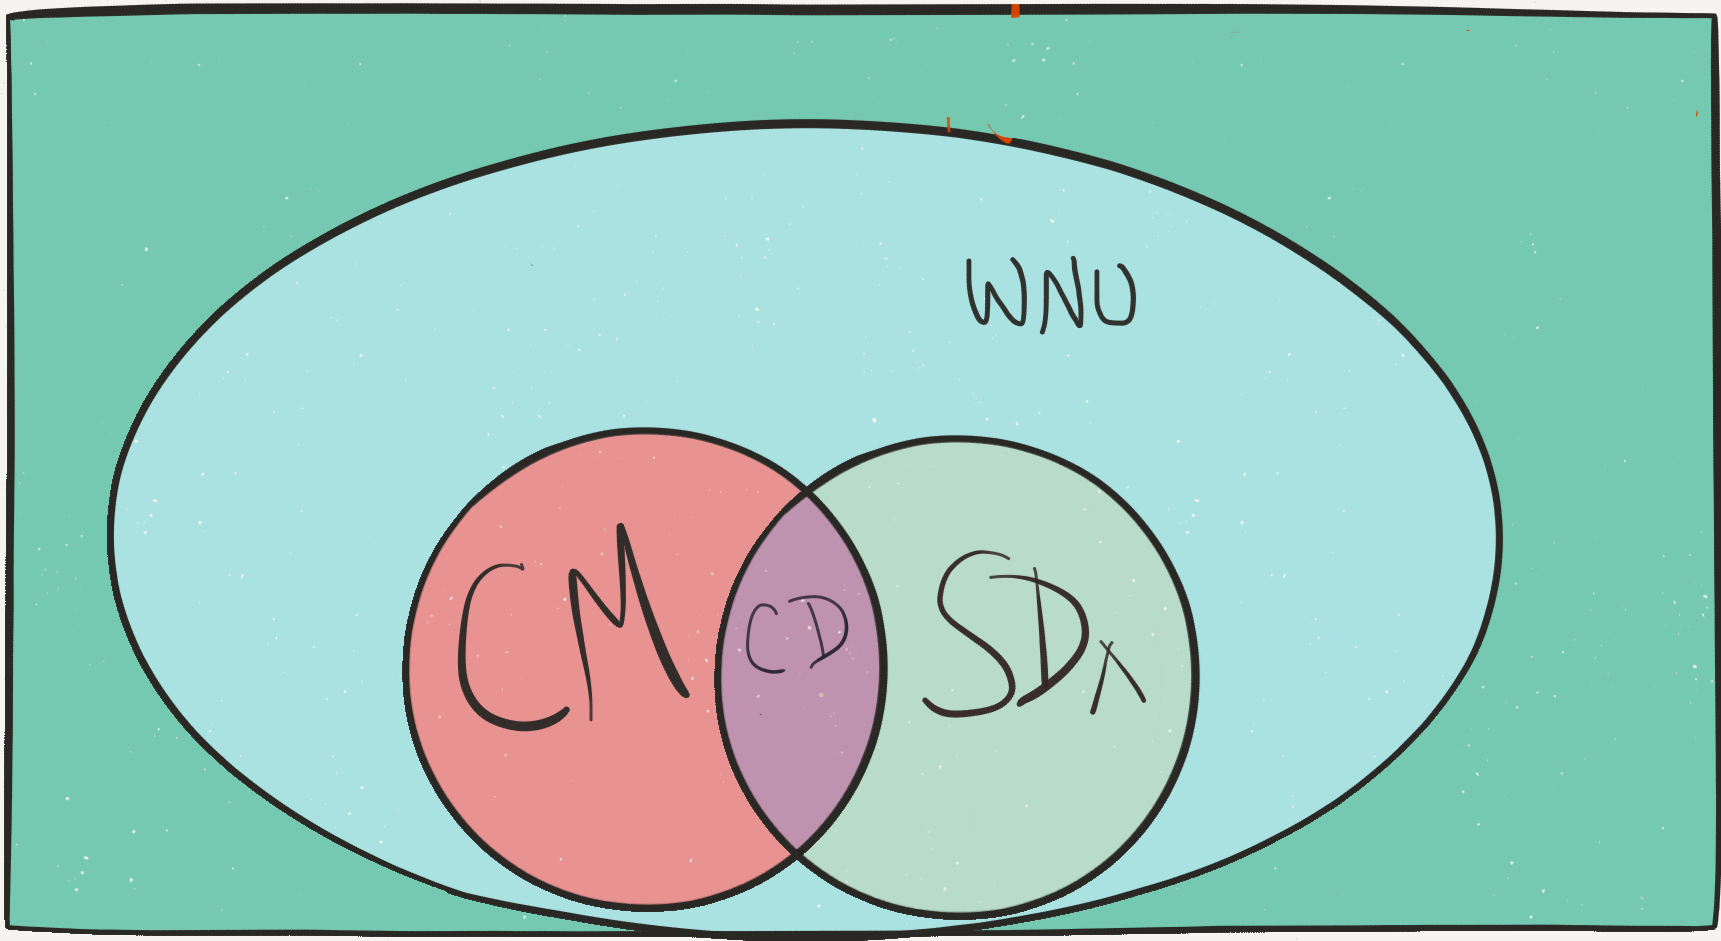
\includegraphics[height=1.5in]{figures/wnu-only-cropped.png}\end{center}
        \onslide<6->\begin{center}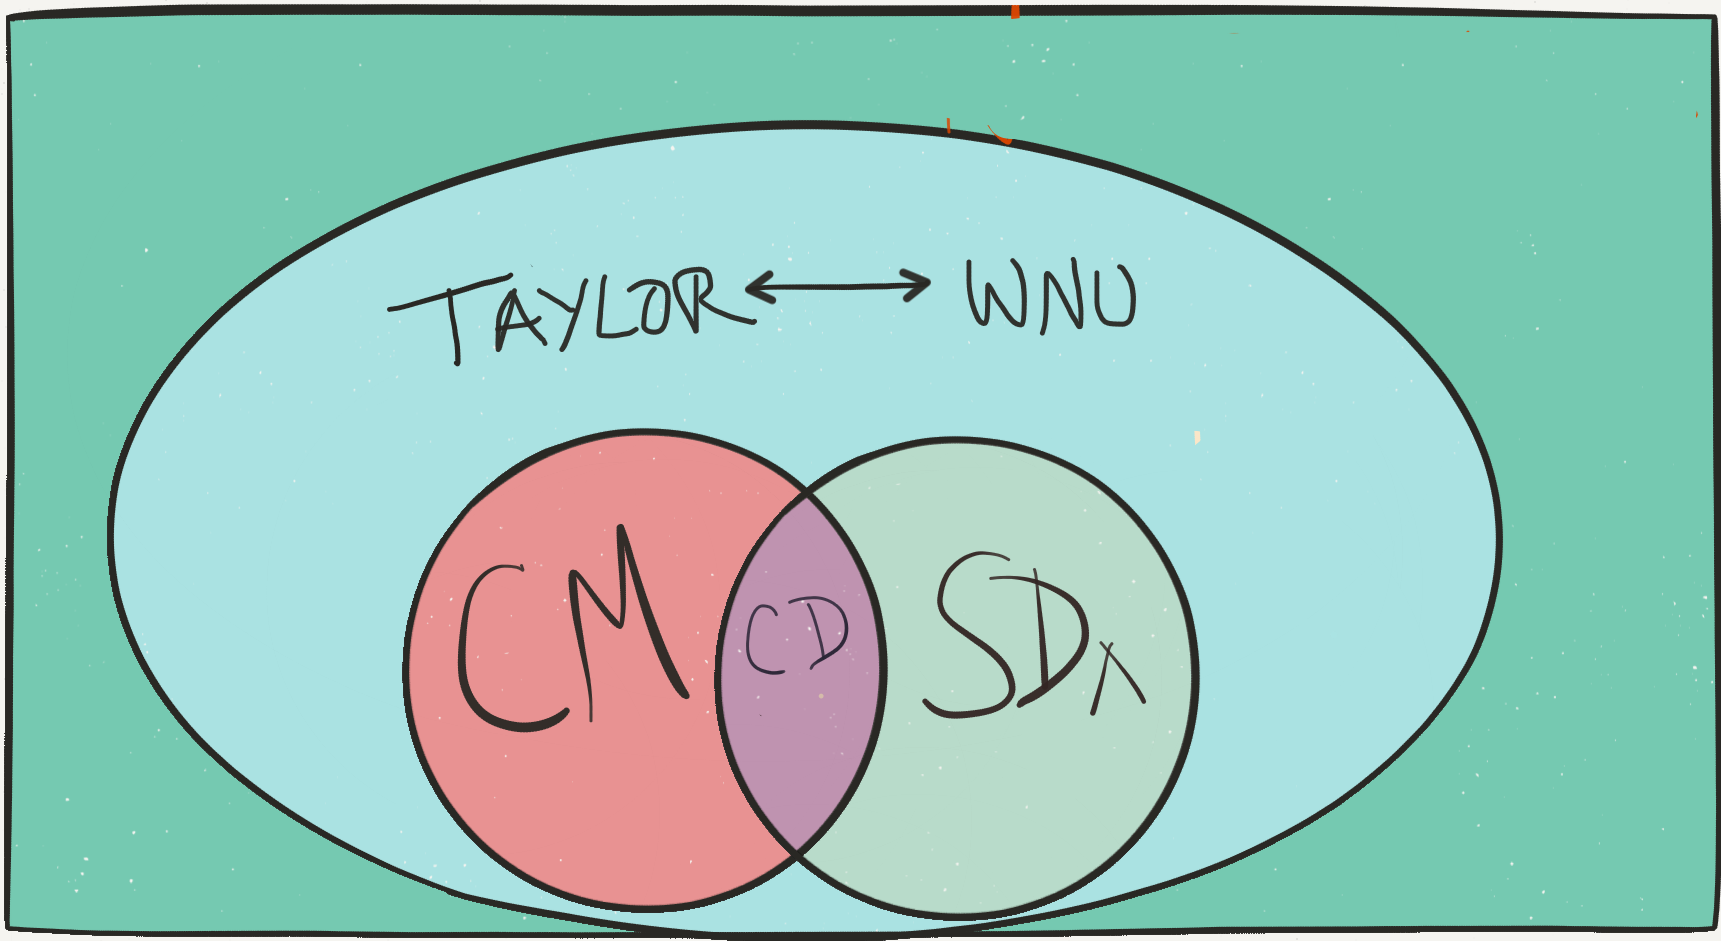
\includegraphics[height=1.5in]{figures/Taylor-cropped.png}\end{center}
        \onslide<7->\begin{center}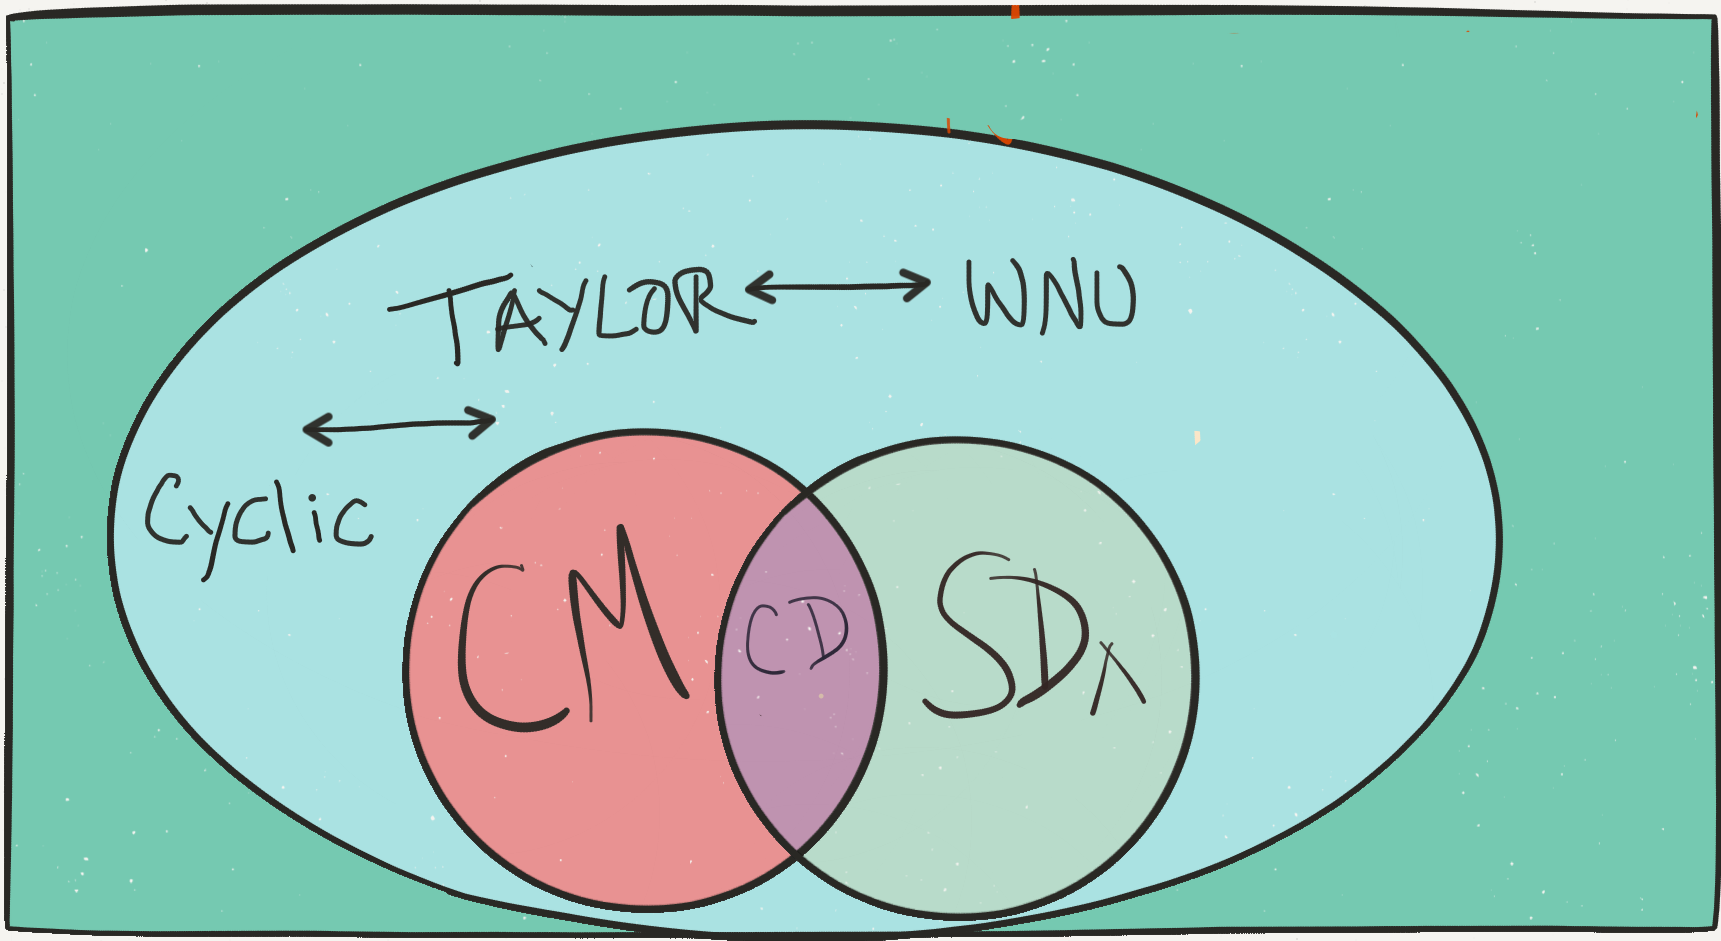
\includegraphics[height=1.5in]{figures/Cyclic-cropped.png}\end{center}
        \onslide<8->\begin{center}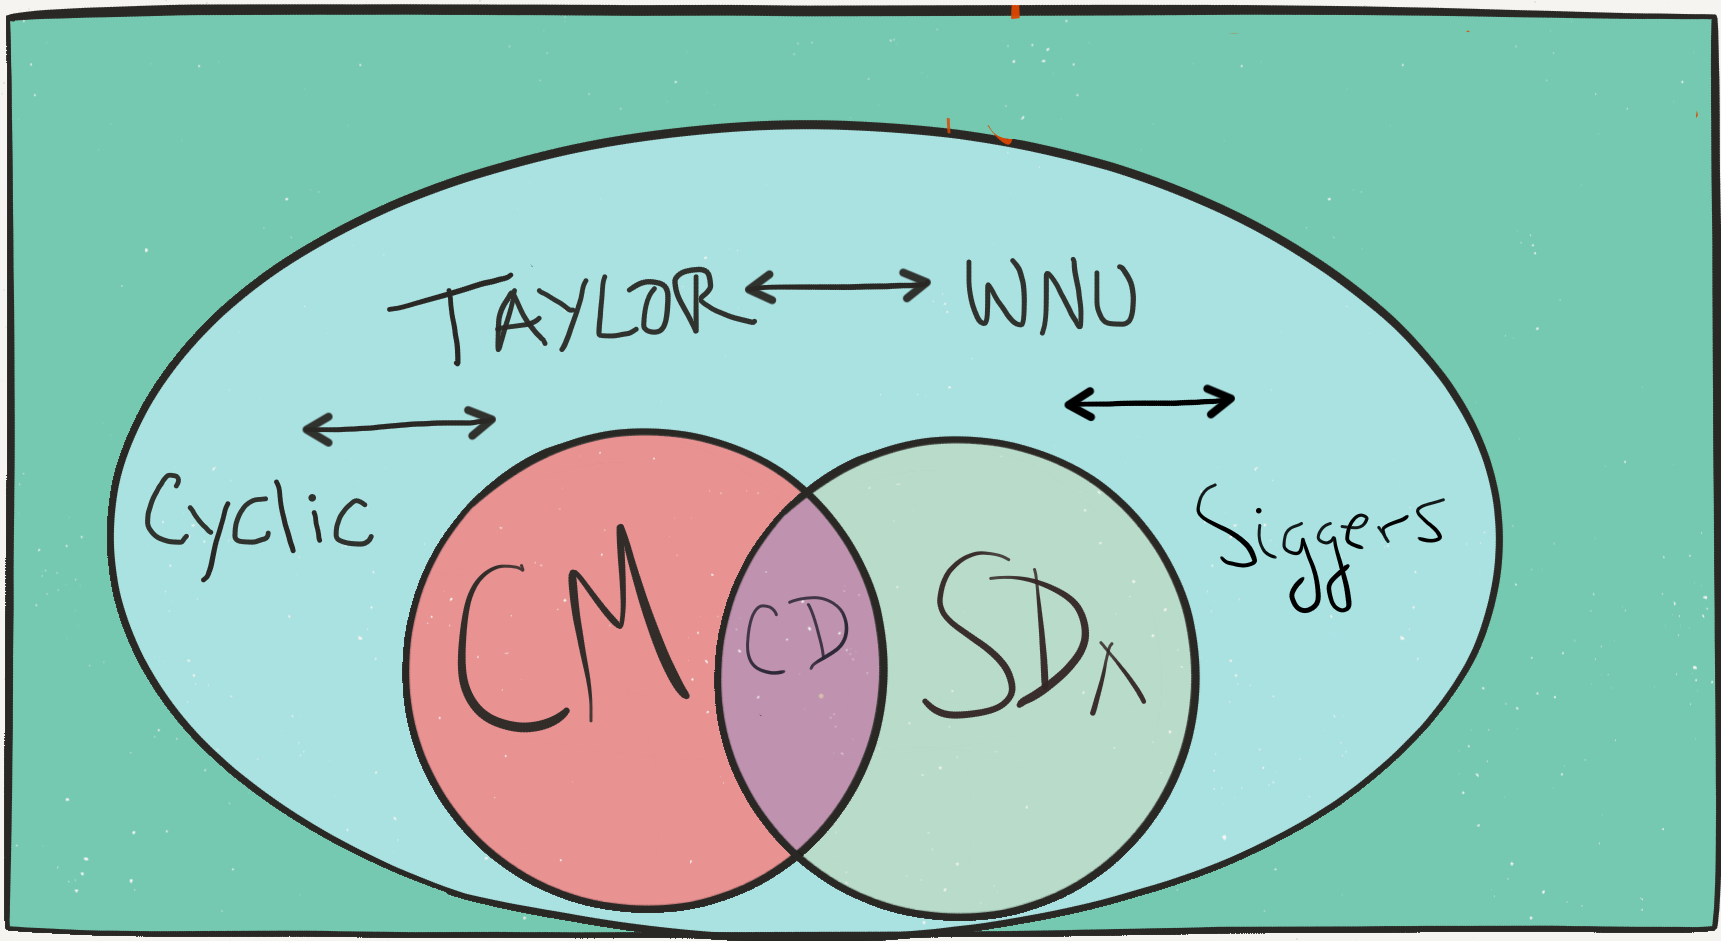
\includegraphics[height=1.5in]{figures/Siggers-cropped.png}\end{center}
        \onslide<9->\begin{center}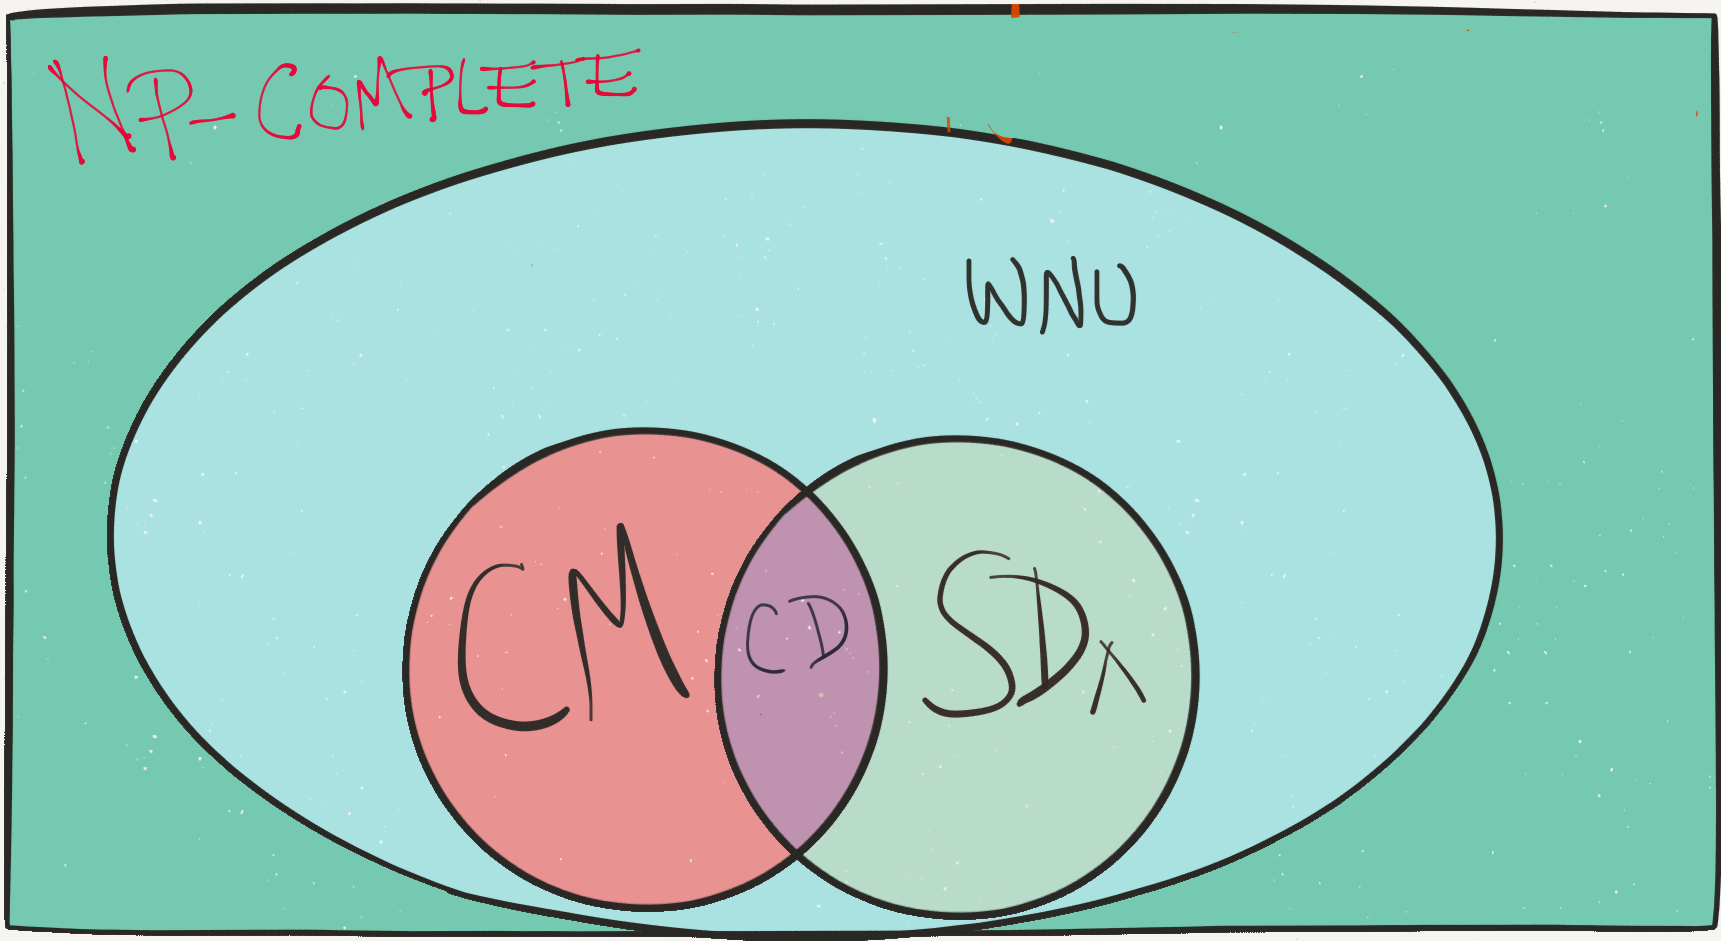
\includegraphics[height=1.5in]{figures/NP-cropped.png}\end{center}
        \onslide<10->\begin{center}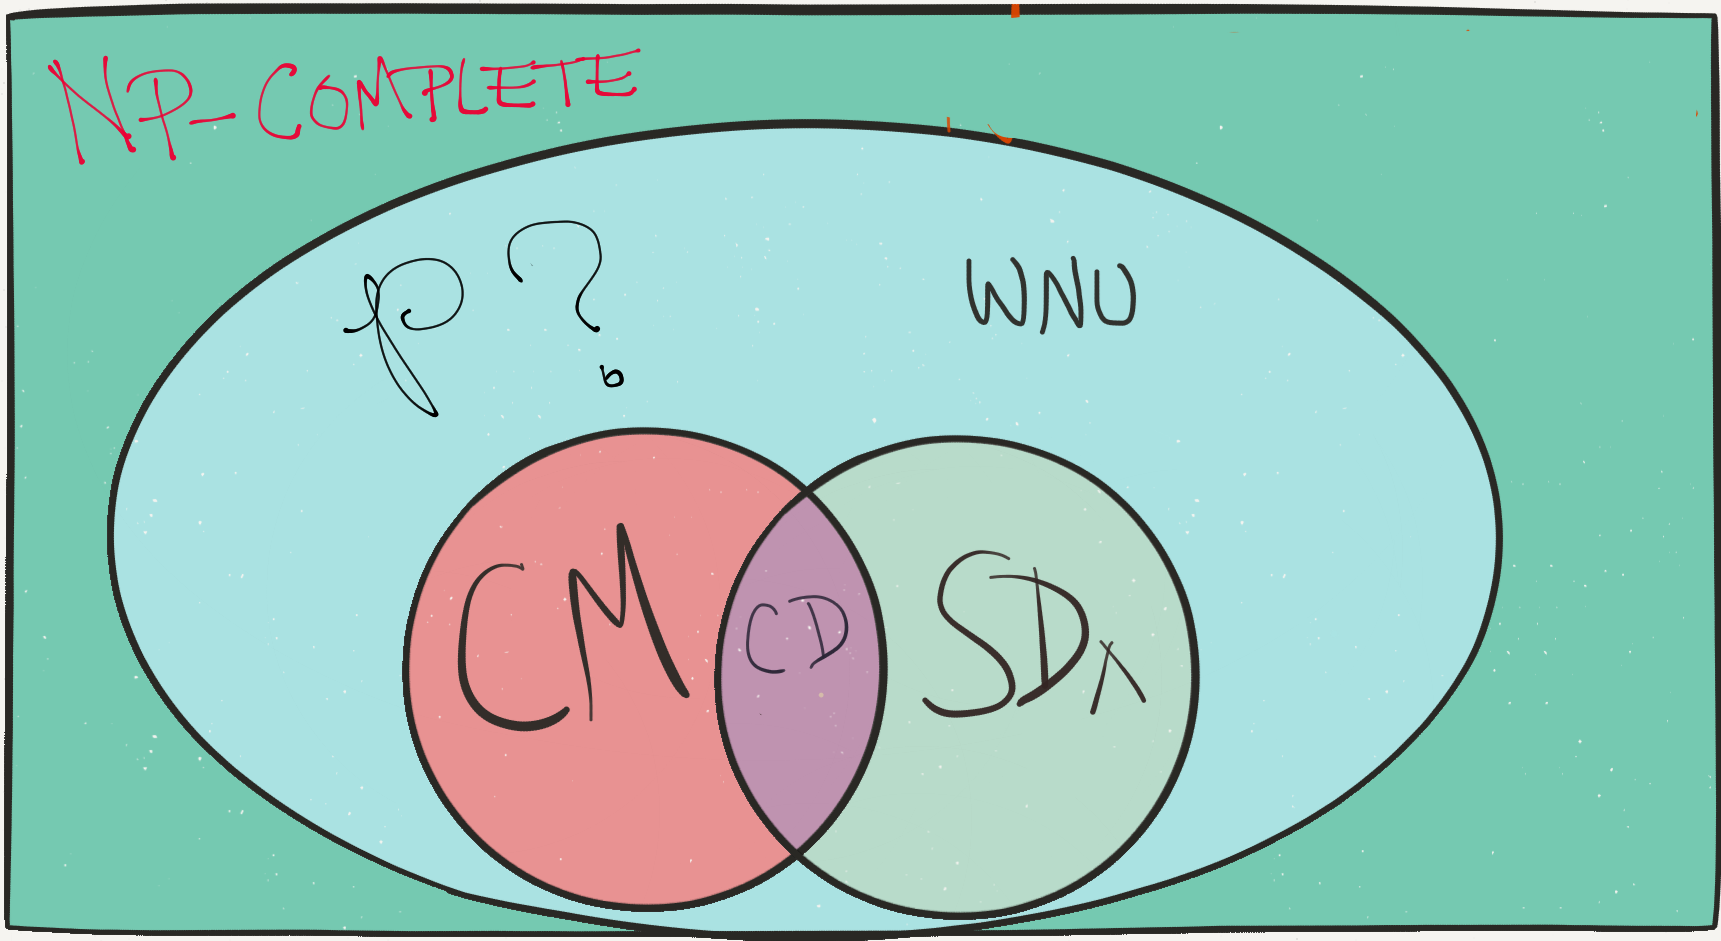
\includegraphics[height=1.5in]{figures/P-cropped.png}\end{center}
      \end{overprint}
}

%%%%%%%%%%%%%%%%%%%%%%%%%%%%%%%%%%%%%%%%%%%%%%%%%%%%%%%%%%%
%% 2: Commutative Idempotent Binars
\frame[label=problem]{
  \frametitle{Commutative Idempotent Binars}
Some more definitions.
  \begin{itemize}
  \item A set $A$ together with a single binary operation is called a \alert{binar}.

  \item A \alert{commutative idempotent binar} is an algebra 
    $\bA = \<A, \cdot\>$ satisfying $x\cdot y \approx y\cdot x$ and $x\cdot x \approx x$.

  \item A binary operation $x\cdot y = t(x,y)$ is a WNU term if and only if it is idempotent and 
    commutative. This suggests the following 
  \end{itemize}
\onslide<2->{
  \begin{block}{Question}
    Is every finite commutative idempotent binar tractable?
  \end{block}
  If the dichotomy conjecture is to hold, then the answer must be ``yes.''
  % We let **\cib** denote the variety of **commutative idempotent binars.**
\\[4pt]
\onslide<3->{
  A semilattice is an associative CIB.\\[4pt]
  Semilattices are tractable (in fact, they have \emph{finite width}).  
}}

}

%%%%%%%%%%%%%%%%%%%%%%%%%%%%%%%%%%%%%%%%%%%%%%%%%%%%%%%%%%%
%% 3: More well known facts

\frame[label=knownfigs]{
  \frametitle{Some well known facts}
  Let $\bA$ be a finite idempotent algebra. Let $\mathbf S_2$ be the 2-elt semilattice.
  %% \begin{block}{}
  \begin{align*}
    \V(\bA) \text{ is CP } &\Longleftrightarrow \quad \bA \text{ has Malcev term}\\
    \onslide<3->{        &\Longrightarrow \quad \bA \text{ has cube term}\\
      \onslide<4->{        &\Longrightarrow \quad \V(\bA) \text{ is CM}\\
        \onslide<5->{        &\Longrightarrow \quad \bS_2 \text{ is not in }
          \V(\bA)
        }
      }
    }
  \end{align*}
  %% \end{block}

  \begin{overprint}
    \onslide<2->
    \begin{center}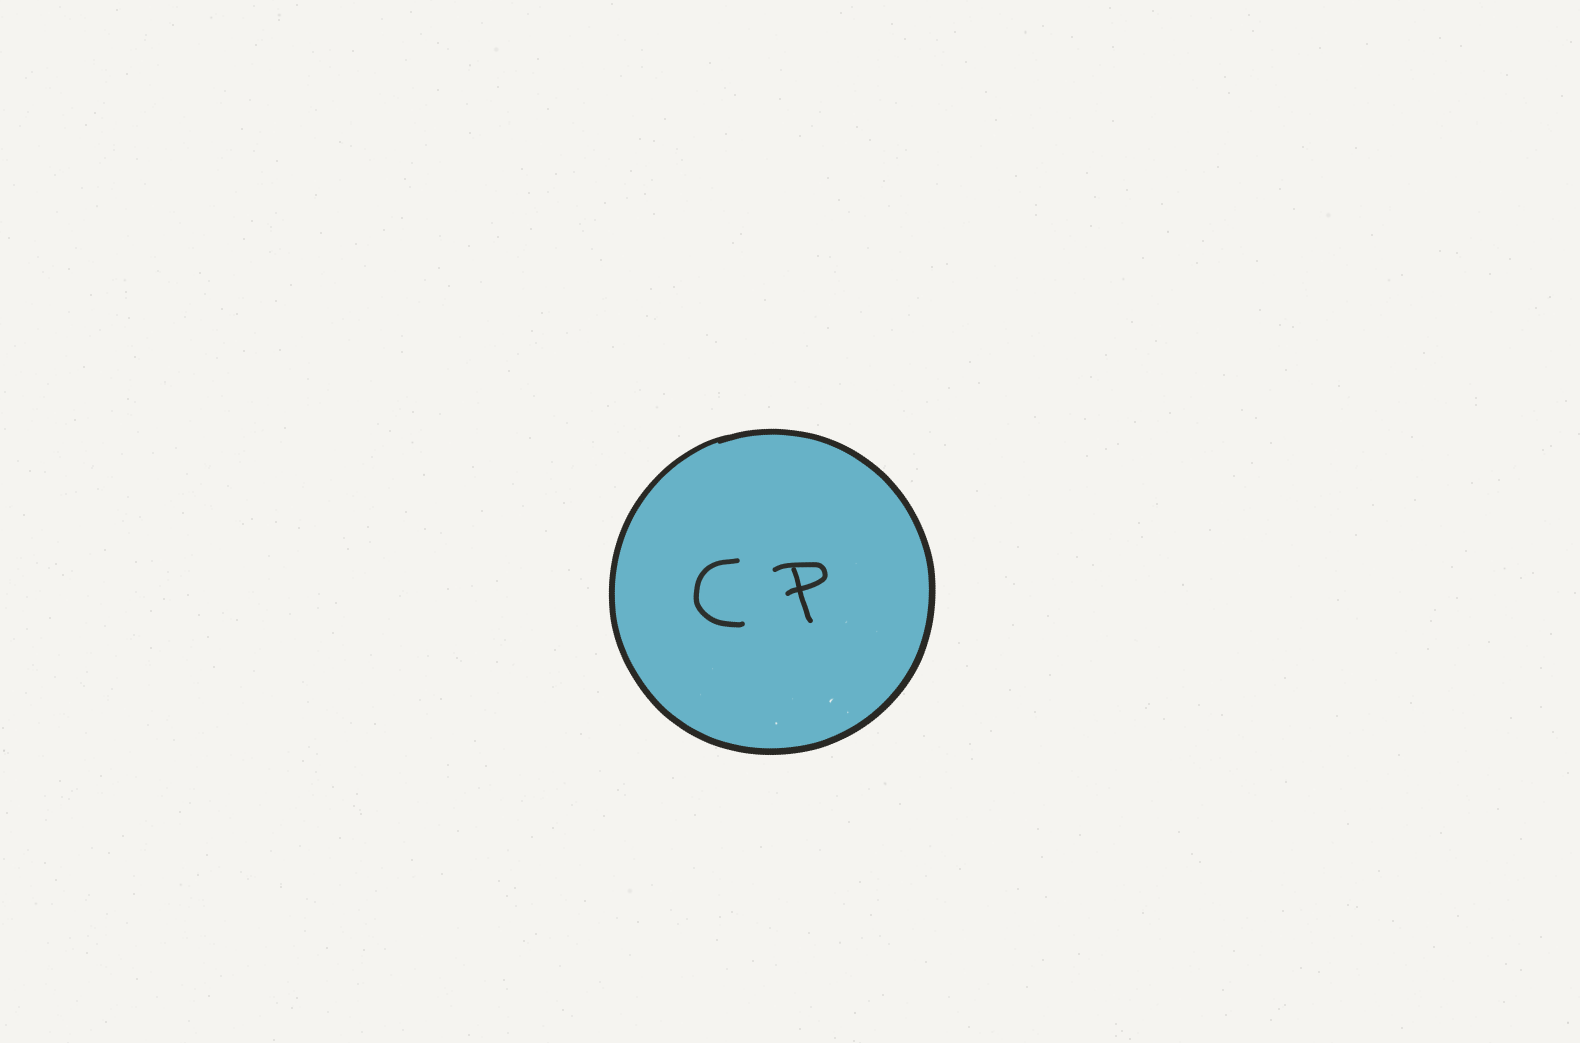
\includegraphics[height=2in]{figures/CP-cropped.png}\end{center}
    \onslide<3->
    \begin{center}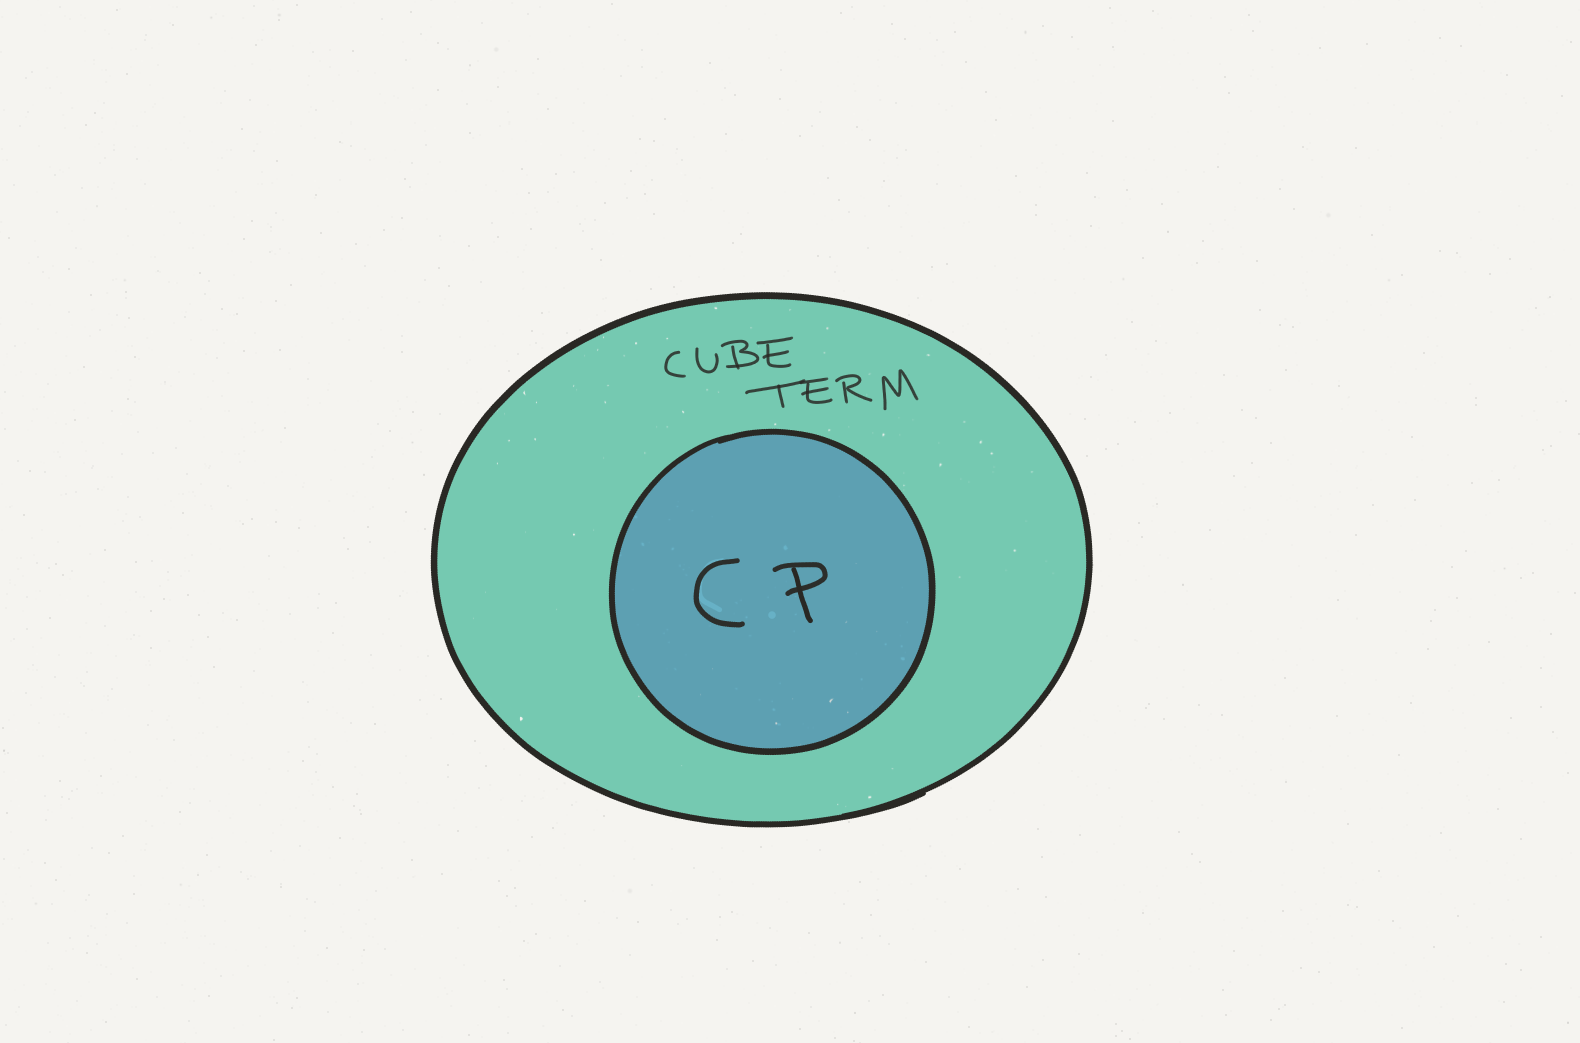
\includegraphics[height=2in]{figures/Cube-cropped.png}\end{center}
    \onslide<4->
    \begin{center}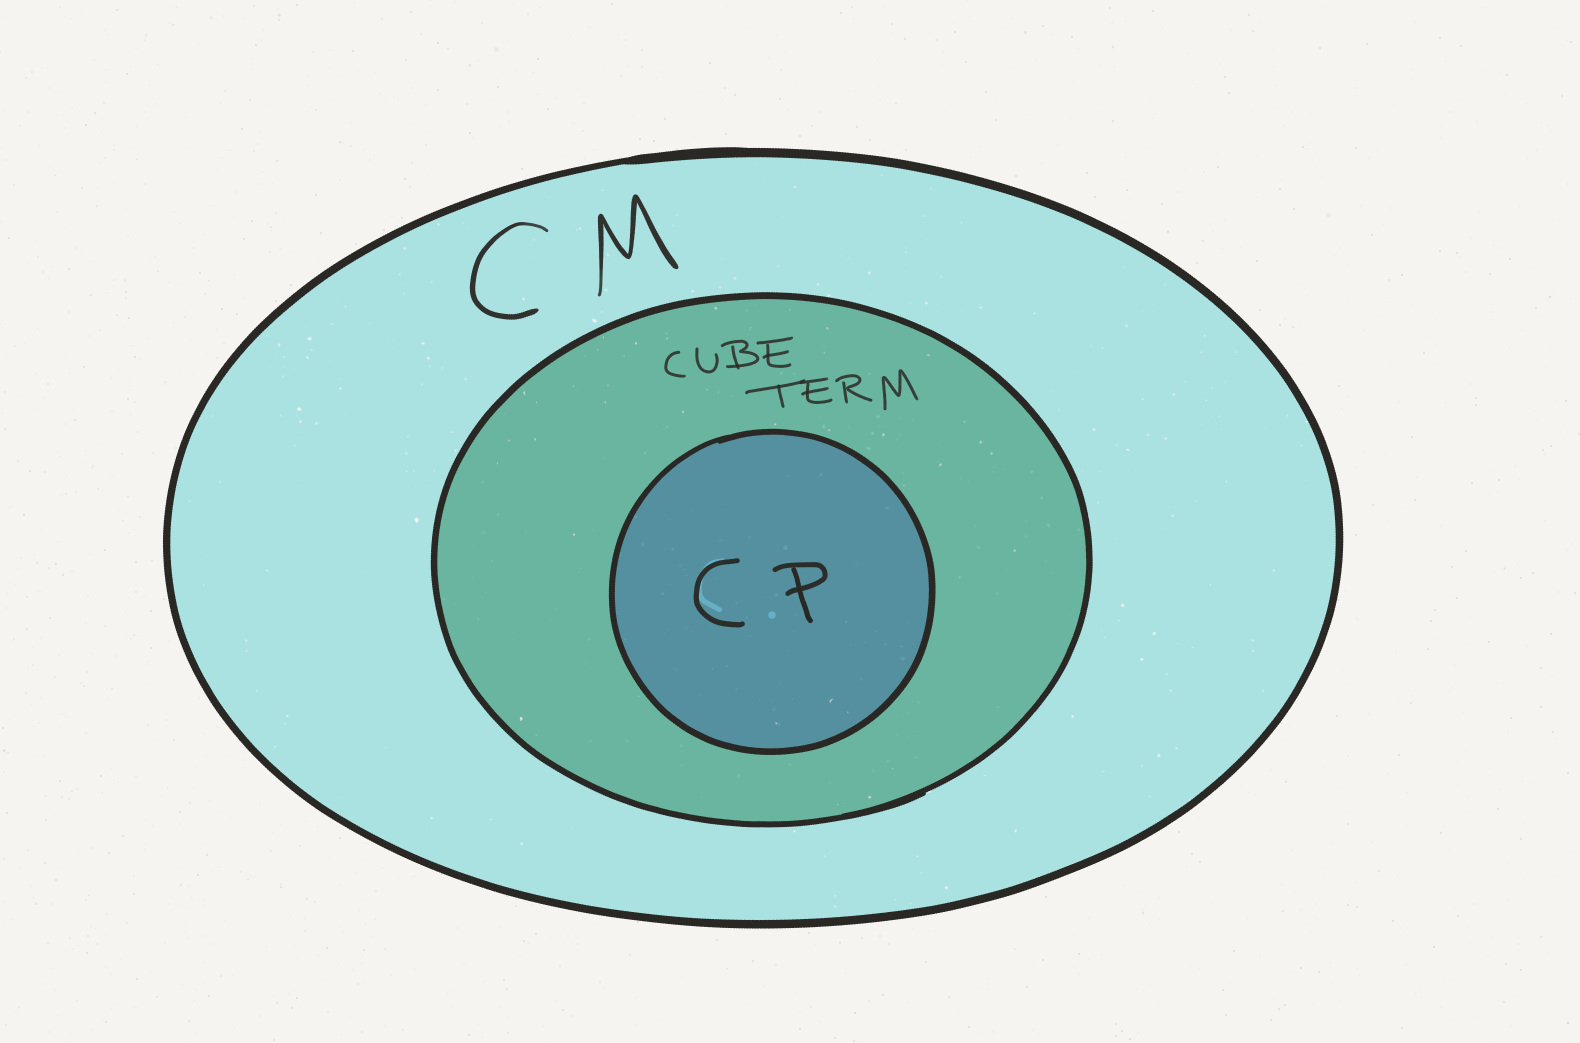
\includegraphics[height=2in]{figures/CM-cropped.png}\end{center}
    \onslide<5->
    \begin{center}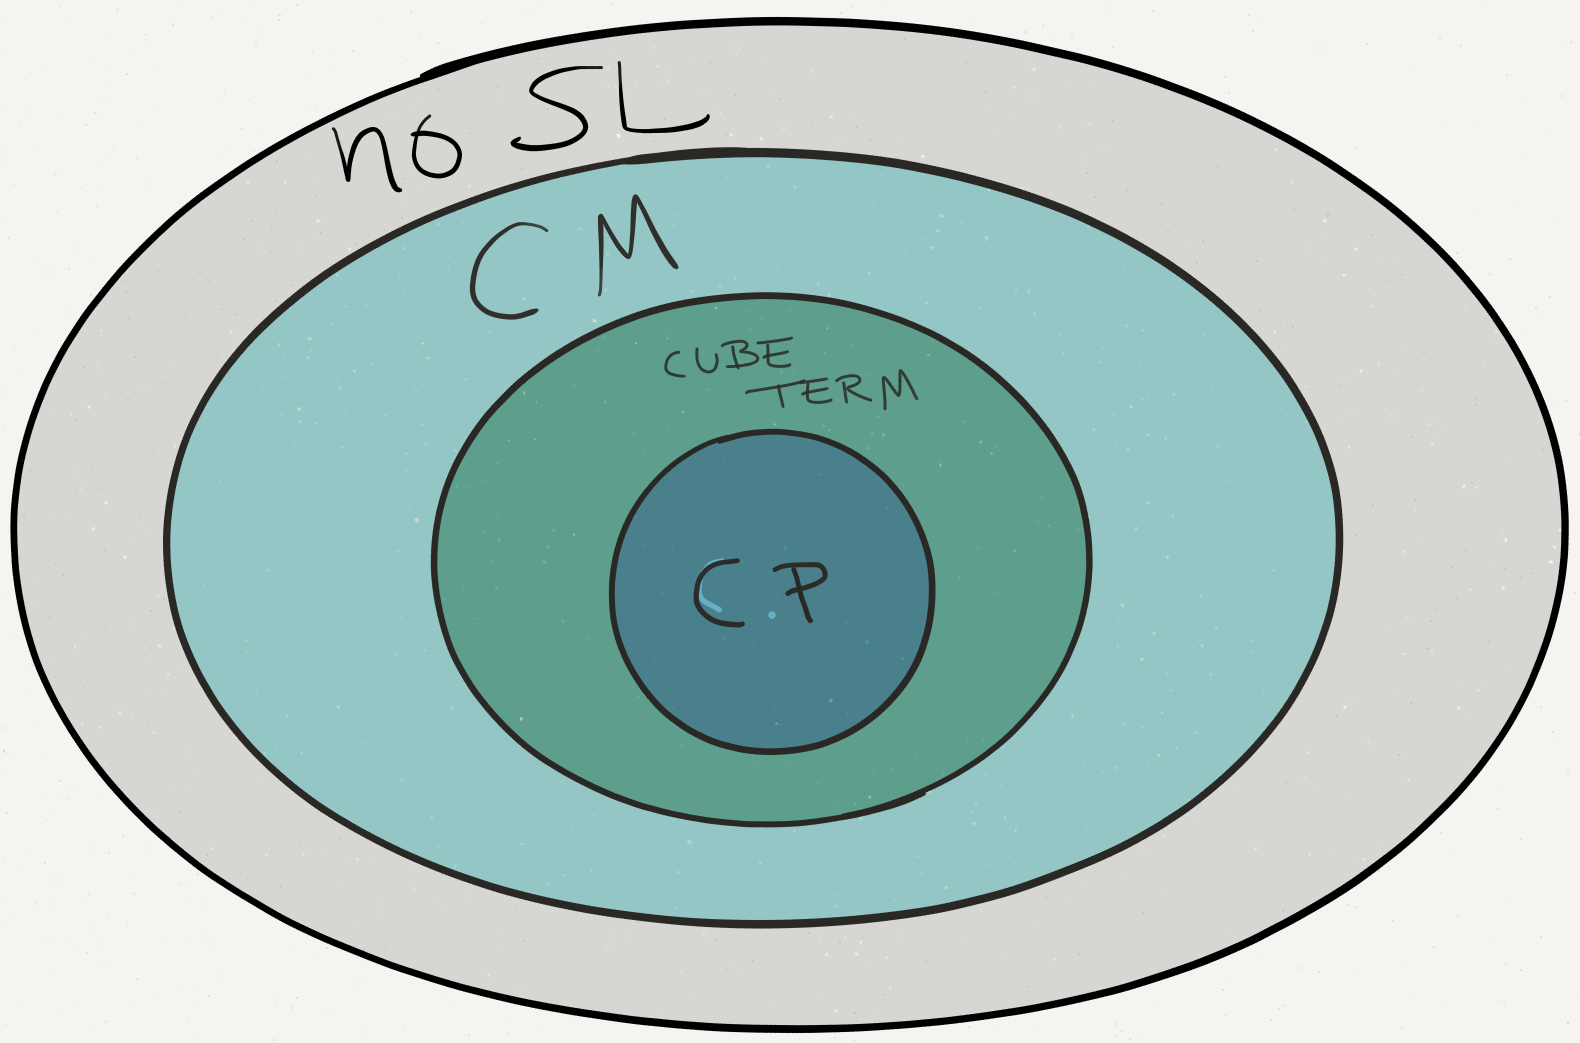
\includegraphics[height=2in]{figures/NoSL-cropped.png}\end{center}
  \end{overprint}
}

%%%%%%%%%%%%%%%%%%%%%%%%%%%%%%%%%%%%%%%%%%%%%%%%%%%%%%%%%%%
%% 4: Some well known facts
\frame[label=known]{
  \frametitle{Some well known facts}

  $\bA=$ a finite idempotent algebra\\[4pt]
  $\mathbf S_2=$ the 2-elt semilattice.

  \begin{align*}
    \V(\bA) \text{ is CP } &\Longleftrightarrow \quad \bA \text{ has a Malcev term}\\
    &\Longrightarrow \quad \bA \text{ has a cube term}\\
    &\Longrightarrow \quad \V(\bA) \text{ is CM}\\
    &\Longrightarrow \quad \bS_2 \text{ is not in } \V(\bA)
  \end{align*}

  \begin{columns}
    \begin{column}{0.4\textwidth}
      \begin{center}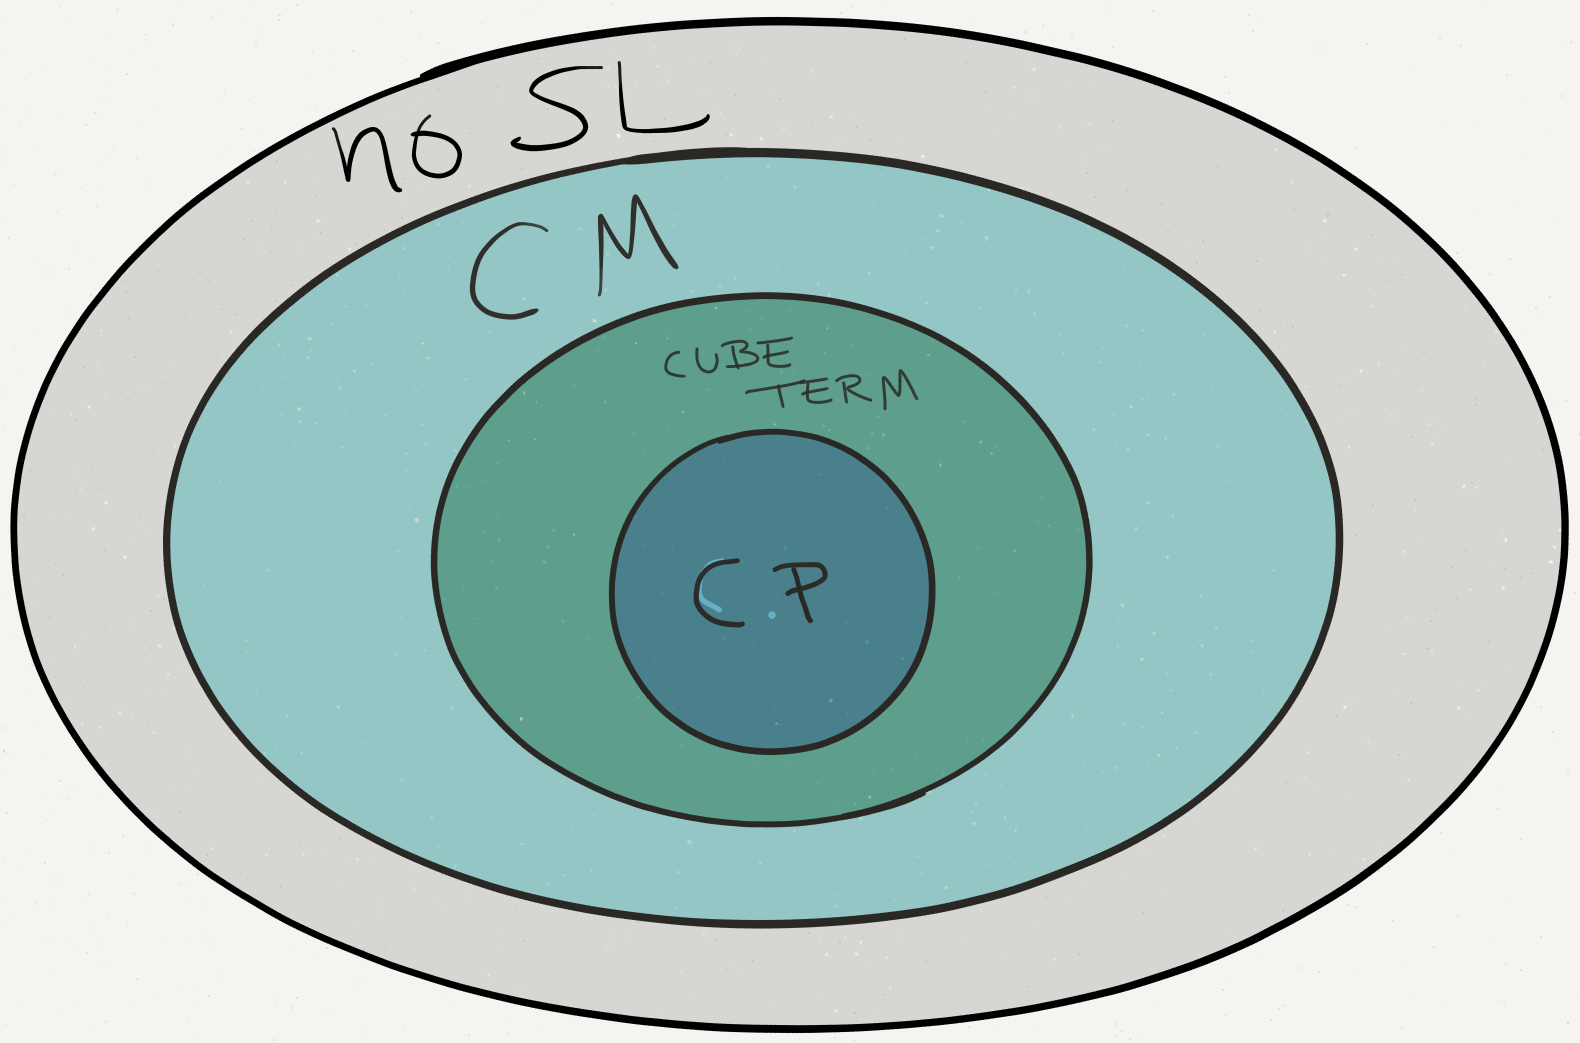
\includegraphics[height=1.25in]{figures/NoSL-cropped.png}\end{center}
    \end{column}
    \begin{column}{0.6\textwidth}
      \begin{itemize}
      \item<2-> cube term $\Longrightarrow$ CM\\[4pt]
        \emph{Proof:} few subalgebras of powers\\[5pt]
        Berman, Idziak, Markovi{\'c}, McKenzie, Valeriote, Willard (BIMMVW) 2010.
        %% ``Varieties with few subalgebras of powers'' 
        \\[10pt]
      \item<3-> CM $\Longrightarrow \; \bS_2$ is not in $\V(\bA)$\\[4pt]
        \emph{Proof:} $\bS_2 \in \V(\bA) \; \Rightarrow\; \bS_2^2 \in \V(\bA)$;\\[4pt]
        ~ \phantom{\emph{Proof:}} $\Con(\bS_2^2)$ is not modular.
      \end{itemize}
    \end{column}
  \end{columns}
}


%%%%%%%%%%%%%%%%%%%%%%%%%%%%%%%%%%%%%%%%%%%%%%%%%%%%%%%%%%%
%% 5
\frame[label=known]{
  \frametitle{Commutative Idempotent Binars (CIBs)}
  Let $\bA$ be a CIB.
  \begin{align*}
    \V(\bA) \text{ is CP } &\Longleftrightarrow \quad \bA \text{ has Malcev term}\\
    &\Longrightarrow \quad \bA \text{ has cube term}\\
    &\Longrightarrow \quad \V(\bA) \text{ is CM}\\
    &\Longrightarrow \quad \bS_2 \text{ is not in } \V(\bA)
  \end{align*}

  \begin{overprint}
    \onslide<1->
    \begin{center}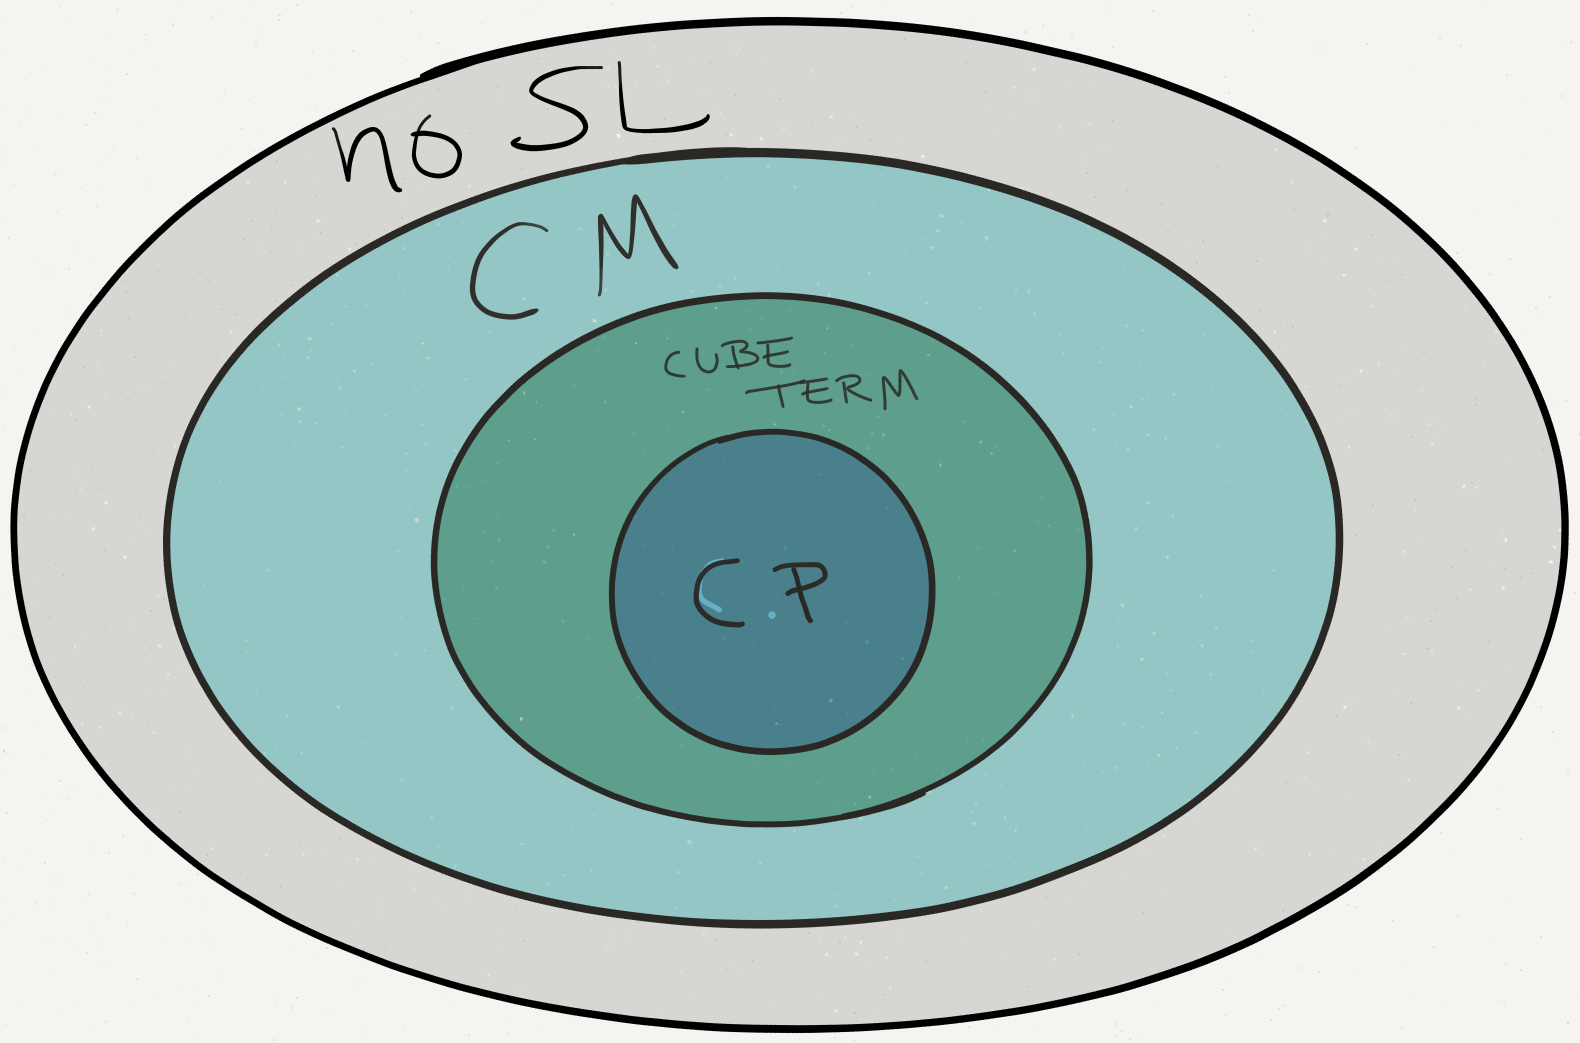
\includegraphics[height=2in]{figures/NoSL-cropped.png}\end{center}
    \onslide<2->
    \begin{center}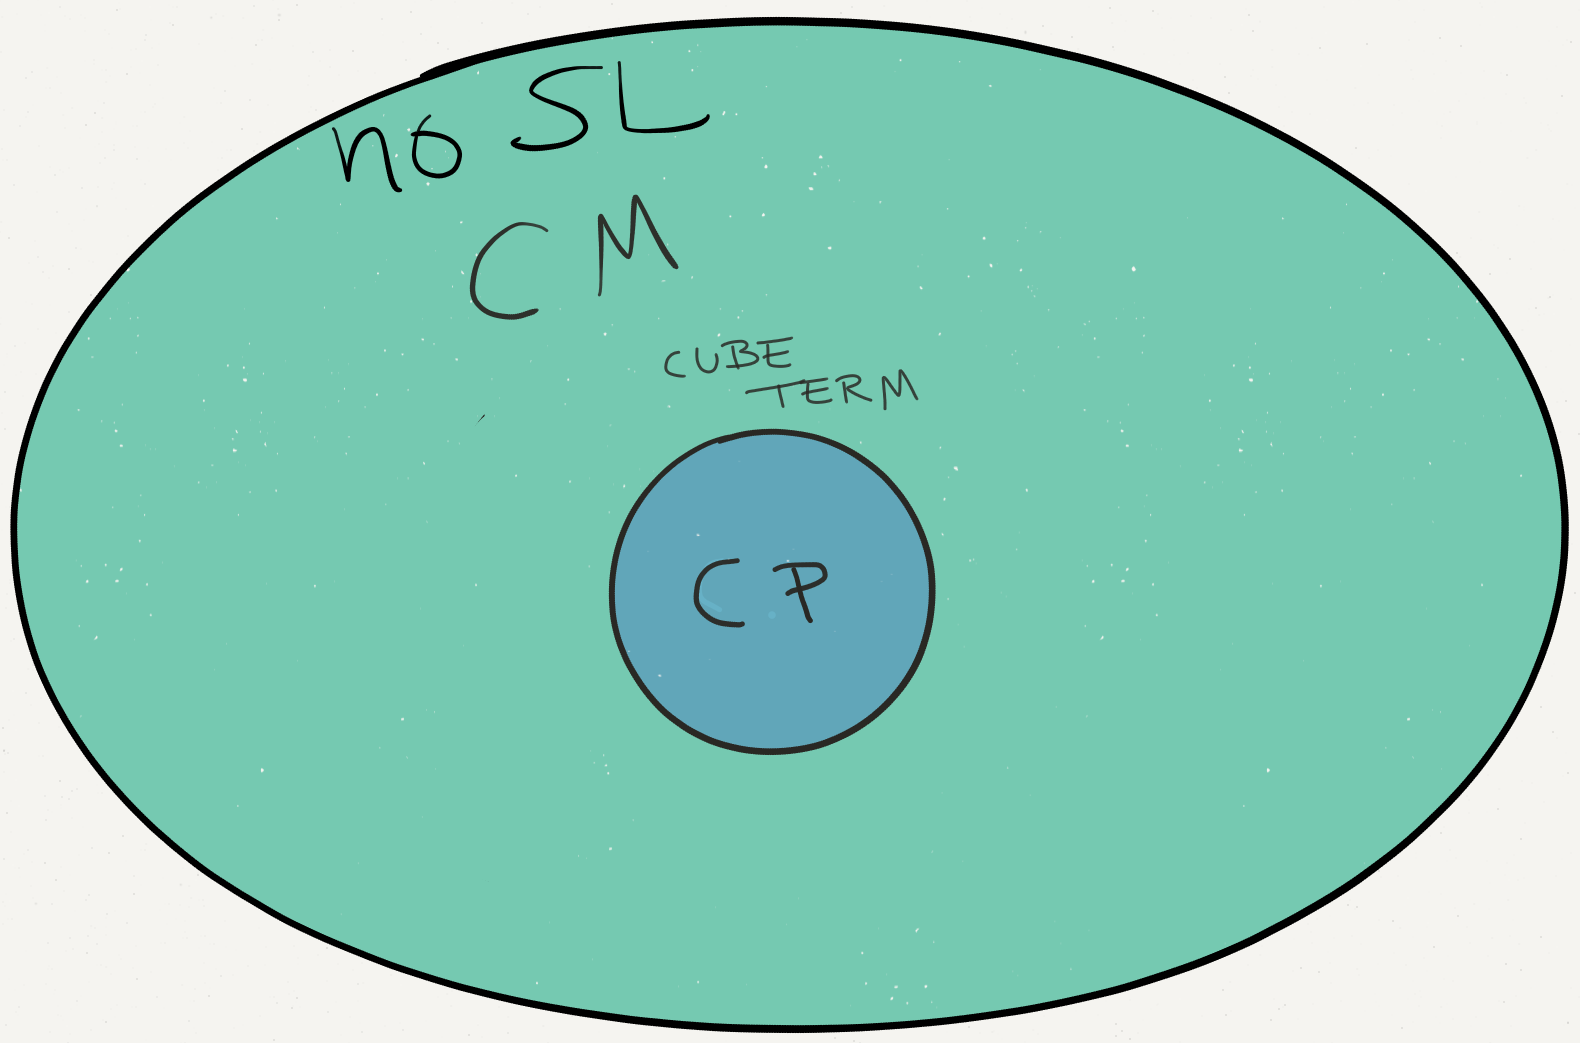
\includegraphics[height=2in]{figures/CubeEquiv-cropped.png}\end{center}
    \onslide<3->
    \begin{center}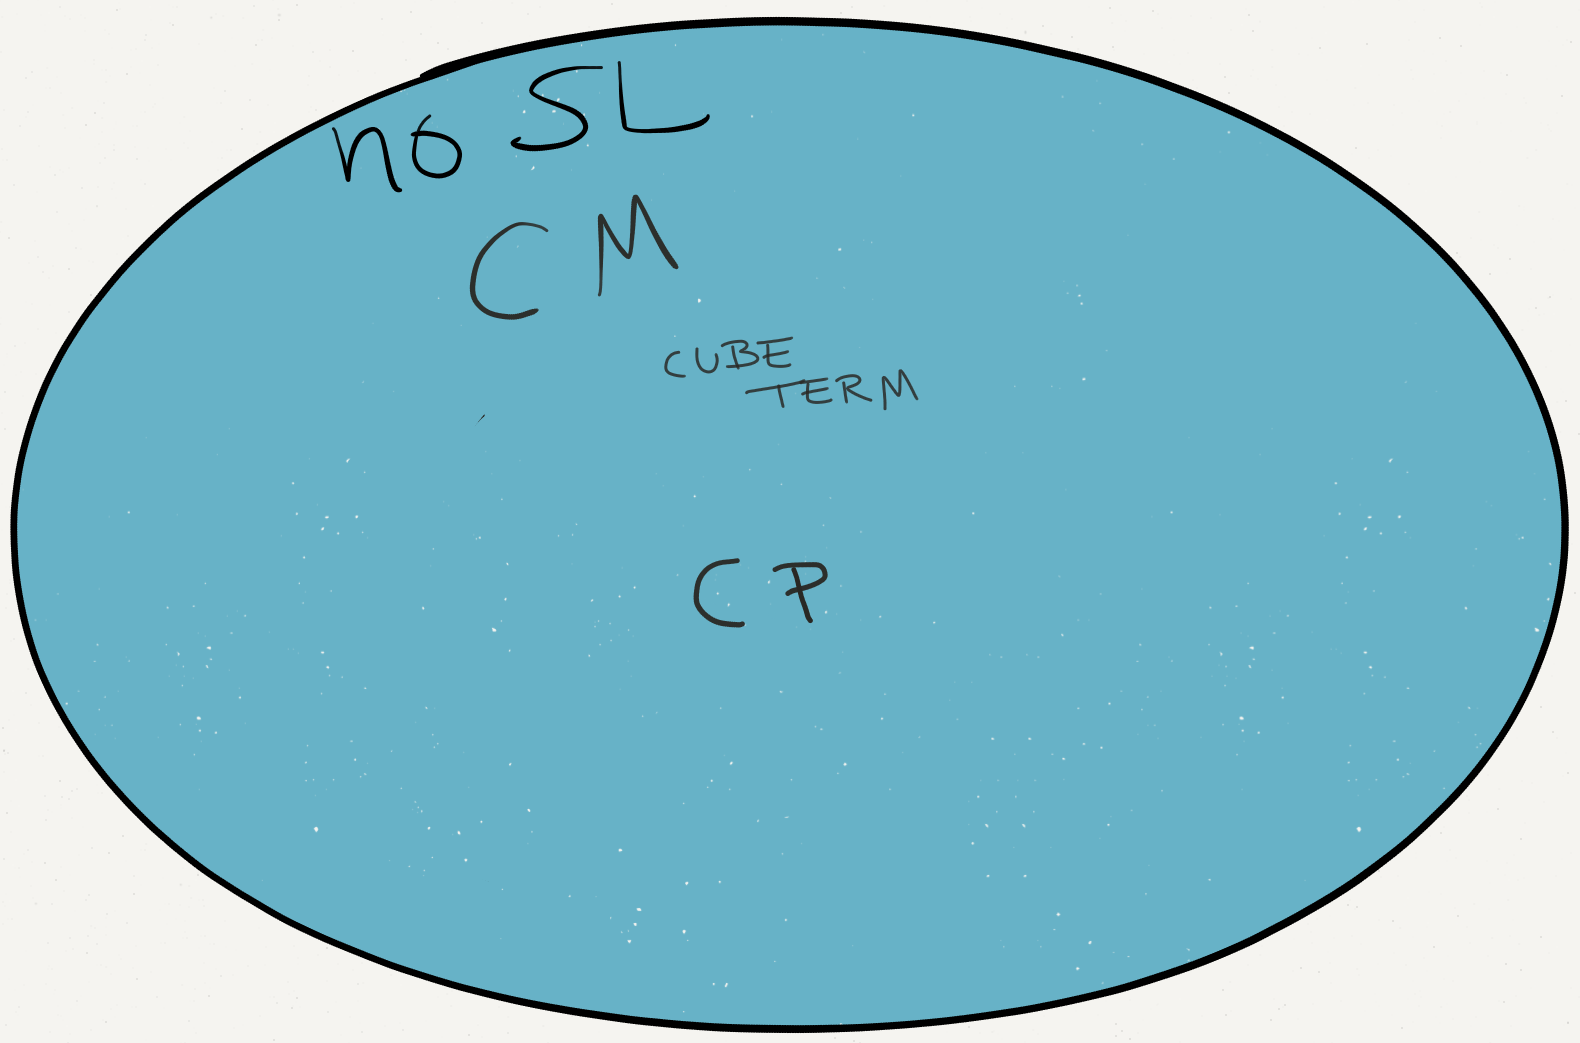
\includegraphics[height=2in]{figures/CPequiv-cropped.png}\end{center}
  \end{overprint}
}




%%%%%%%%%%%%%%%%%%%%%%%%%%%%%%%%%%%%%%%%%%%%%%%%%%%%%%%%%%%
%% 6
\frame[label=cube]{
  \frametitle{Cube Terms}
  \begin{block}{}
    A \alert{cube operation} is
    a function $c: A^n \rightarrow A$ satisfying
    for each $1 \leq i \leq n$ 
    $c(w_1, \dots, w_n) = x$ where 
    $\{w_1, \dots, w_n\} \subseteq \{x, y\}$ and 
    $w_i = y$.
    \\[4pt]
    Here $x$ and $y$ are distinct variables.
    \\[6pt]
    An algebra $\bA$ is said to have a \alert{cube term} if its clone
    of term operations contains a cube operation. 
  \end{block}
  \vfill
  \onslide<2->{
    Cube terms were introduced in... ?\\[8pt]
    Berman, Idziak, Markovi{\'c}, McKenzie, Valeriote, Willard,\\
    ``Varieties with few subalgebras of powers,'' 2010. \\[10pt]
    Markovi{\'c}, Mar{\'o}ti, McKenzie,\\
    ``Finitely related clones \& algebras with cube terms,'' 2012.}
}


%%%%%%%%%%%%%%%%%%%%%%%%%%%%%%%%%%%%%%%%%%%%%%%%%%%%%%%%%%%
%% 4
\frame[label=cube]{
  \frametitle{Cube Term Blockers}
  \begin{block}{}
    %% \begin{definition}
    A \alert{cube term blocker} (CTB) for $\bA$ is a pair $(C, B)$ of subuniverses
    of $\bA$ satisfying $\emptyset < C < B \leq A$ and for every term 
    $t(x_1, \dots, x_n)$ of $\bA$ there is an index $i \in [n]$ such that 
    \[
    (\forall (b_1, \dots, b_n) \in B^n) (b_i \in C \longrightarrow t(b_1, \dots, b_n)\in C).
    \]
  \end{block}
  %% \end{definition}
  %% We call a set $D$ a (proper) \defn{ideal} of a \cib $\bA = \< A, \cdot\>$
  %%   if $D$ is a (proper) subset of $A$ satisfying $d\cdot a \in D$ for all 
  %% $d\in D$ and $a \in A$.
  Markovi{\'c}, Mar{\'o}ti, McKenzie proved that a finite idempotent algebra has
  a cube term iff it possesses no CTB.  

  \vfill
  \onslide<2->{
    \begin{lemma}
      A finite CIB $\bA = \<A, \cdot\>$ has a CTB if and only if 
      $\bS_2 \in \sansH \sansS (\bA)$.
    \end{lemma}
    \onslide<3->{
      \begin{proof}
        If $(C, B)$ is a CTB, then $\theta = C^2 \cup (B- C)^2$ is a congruence of
        $\bB = \<B, \cdot\>$ and $\bB/\theta \cong \bS_2$. 
        \\[5pt]
        Conversely, suppose $\bS_2 \in \sansH \sansS (\bA)$, and $\bB$ is 
        a subalgebra of $\bA$ with $\bB/\theta$ a meet-SL for some $\theta$. 
        Let $C/\theta$ be the bottom of $\bB/\theta$, then $(C, B)$ is a CTB.
      \end{proof}
    }
}}


}



  %%%%%%%%%%%%%%%%%%%%%%%%%%%%%%%%%%%%%%%%%%%%%%%%%%%%%%%%%%%
  %% 4
  \frame[label=cube]{
    \frametitle{Collapse for CIBs}

    Kearnes and Tschantz,
    ``Automorphism groups of squares and of free algebras,'' 2007.

    \begin{lemma}
      If $V$ is an idempotent variety that is not congruence permutable, then there
      are subuniverses $U$ and $W$ of $\bF := \bF_V\{x, y\}$ (the 2-generated free
      algebra) satisfying 
      \begin{enumerate}[1.]
      \item $x\in U \cap W$
      \item $y \in U^c \cap W^c$
      \item $(U \times F) \cup (F \times W) \leq \bF^2$
      \end{enumerate}
    \end{lemma}
    \onslide<2->{
      For CIB's, $U$ or $W$ will be an ideal.\\[4pt]
      This implies a CTB and a semilattice.}
  }

  %%%%%%%%%%%%%%%%%%%%%%%%%%%%%%%%%%%%%%%%%%%%%%%%%%%%%%%%%%%
  %% 4
  \frame[label=examples]{
    \frametitle{Remaining Question for CIBs}

    \begin{block}{Conclusion}
      Let $\bA$ be a CIB and $\bS_2 \notin \V(\bA)$. Then $\CSP(\bA)$ is tractable.
    \end{block}

    \onslide<2->
    \begin{block}{Open Question}
      Let $\bA$ be a CIB and $\bS_2 \in \V(\bA)$.  Is $\CSP(\bA)$ tractable?
    \end{block}

    Recall, for every $\bA$, 
    \begin{itemize}
    \item<3->if $\bS_2 \in \V(\bA)$, then $\V(\bA)$ is not CM;

    \item<4-> if $\V(\bA)$ is  $\mathrm{SD}_\wedge$, then $\CSP(\bA)$ is
    tractable (in fact, always has a solution).
    \end{itemize}

    \onslide<5->
    \begin{block}{Revised Question}
    Let $\bA$ be a CIB with $\bS_2$ in $\V(\bA)$, not $\mathrm{SD}_\wedge$.
    Is $\CSP(\bA)$ tractable?
    \end{block}

  }

  %%%%%%%%%%%%%%%%%%%%%%%%%%%%%%%%%%%%%%%%%%%%%%%%%%%%%%%%%%%
  %% 4
  \frame[label=examples]{
    \frametitle{Examples}

    \begin{tabular}{c|cccc}
$\cdot$ & 0 & 1 & 2 & 3\\
\hline
      0 & 0 & 0 & 0 & 1\\
      1 & 0 & 1 & 3 & 2\\
      2 & 0 & 3 & 2 & 1\\
      3 & 1 & 2 & 1 & 3\\
    \end{tabular}
\hskip1cm
    \begin{tabular}{c|cccc}
$\ast$ & 0 & 1 & 2 & 3\\
\hline
      0 & 0 & 0 & 1 & 1\\
      1 & 0 & 1 & 3 & 2\\
      2 & 1 & 3 & 2 & 1\\
      3 & 1 & 2 & 1 & 3\\
    \end{tabular}
\vskip1cm
  \begin{columns}
    \begin{column}{0.4\textwidth}
    \begin{tabular}{c|cccc}
$\circ$ & 0 & 1 & 2 & 3\\
\hline
      0 & 0 & 0 & 2 & 1\\
      1 & 0 & 1 & 3 & 2\\
      2 & 2 & 3 & 2 & 1\\
      3 & 1 & 2 & 1 & 3\\
    \end{tabular}
    \end{column}
    \begin{column}{0.5\textwidth}
    Maroti's idea:
    \vskip1cm
    Bergman's idea: replace basic binary operation with a term from
    $\Clo(\bA)$, say $t(x,y) = (x\ast y) \ast x$.\\[4pt] If $\<A, t\>$ tractable,
    then so is $\<A, \ast\>$
    \end{column}
  \end{columns}
  }

    \end{document}




    Question: Does the converse of the last implication hold in general?
    That is, if A is an finite idempotent algebra, then is it true that

    S not in V(A)  =>  V(A) is CM?

    This is certainly not true. For example, take A to be a 2-element set. However,
    even if you omit type 1 it fails. Example 2.2 in the Freese-McKenzie paper on
    Robust Maltsev conditions is an example. (It is actually an example due to
    Matt.) You can probably find more examples by hunting through the Berman-Burris
    catalog of 3-element binars:
    http://www.math.uic.edu/~berman/1994-Groupoid-Catalog-Preprint.pdf 

    It seems to me this is what Prop 3.9 and Cor 3.10 of Freese-Valeriote
    says.  (If not, do you know a counter-example?)
    No, the stuff about the tails is subtle. That's what Matt's example was designed to show.

    I should know counter-examples for each of the converses that don't
    hold.  Right now, I only know of one for "CM => cube term".  Namely,
    the algebra Kearnes4.ua available here:

    https://github.com/UACalc/AlgebraFiles/tree/master/Kearnes

    has no cube term, but V(A) is CM.
    This is the only example I am aware of.

    What are examples of algebras with a cube term but no Malcev term.  (I
    should know this! ...Jiali, feel free to jump in here!)
    Every near-unanimity term is a cube term. So Lattices, for example, have cube terms but not Malcev terms. Also, the gmm terms of Dalmau are cube terms. I presume they are not always Malcev terms.

    Now, back to the CIB case.  Once we prove (for CIBs) that

    S not in V(A)  =>   V(A) is CP

    then all the conditions above are equivalent.  That is,

    For a finite CIB A, TFAE

    1. V(A) is CP
    2. A has a Malcev term
    3. A has a cube term
    4. V(A) is CM
    5. S is not in V(A)
    Correct. By the way, do we need A finite for this? I suspect not







